\begin{enumerate}
\item Your printer has been pre-calibrated and tested; however, after unpacking you will need to double check that everything is in order before you print.

\item You should set your printer on a stable, flat, and level surface large enough for extra space around the printer. Make sure your printer work space is clear of anything that could obstruct the movement of the printer. \textcolor{red}{Make sure there are no flammable fabrics or liquids near the printer space}. It is also best to not put your printer near a drafty window or air conditioner vent.

\index{end stops}
\item Check that the three mechanical end stops are aligned to contact with the respective ends. The mechanical end stops are small switches located at the home point of each axis.
(Fig. \ref{fig:axes}, page \pageref{fig:axes}; Fig. \ref{fig:xz_endstops}, page \pageref{fig:xz_endstops}; Fig. \ref{fig:y_endstop}, page \pageref{fig:y_endstop}).
\begin{figure}[hp]
\centering
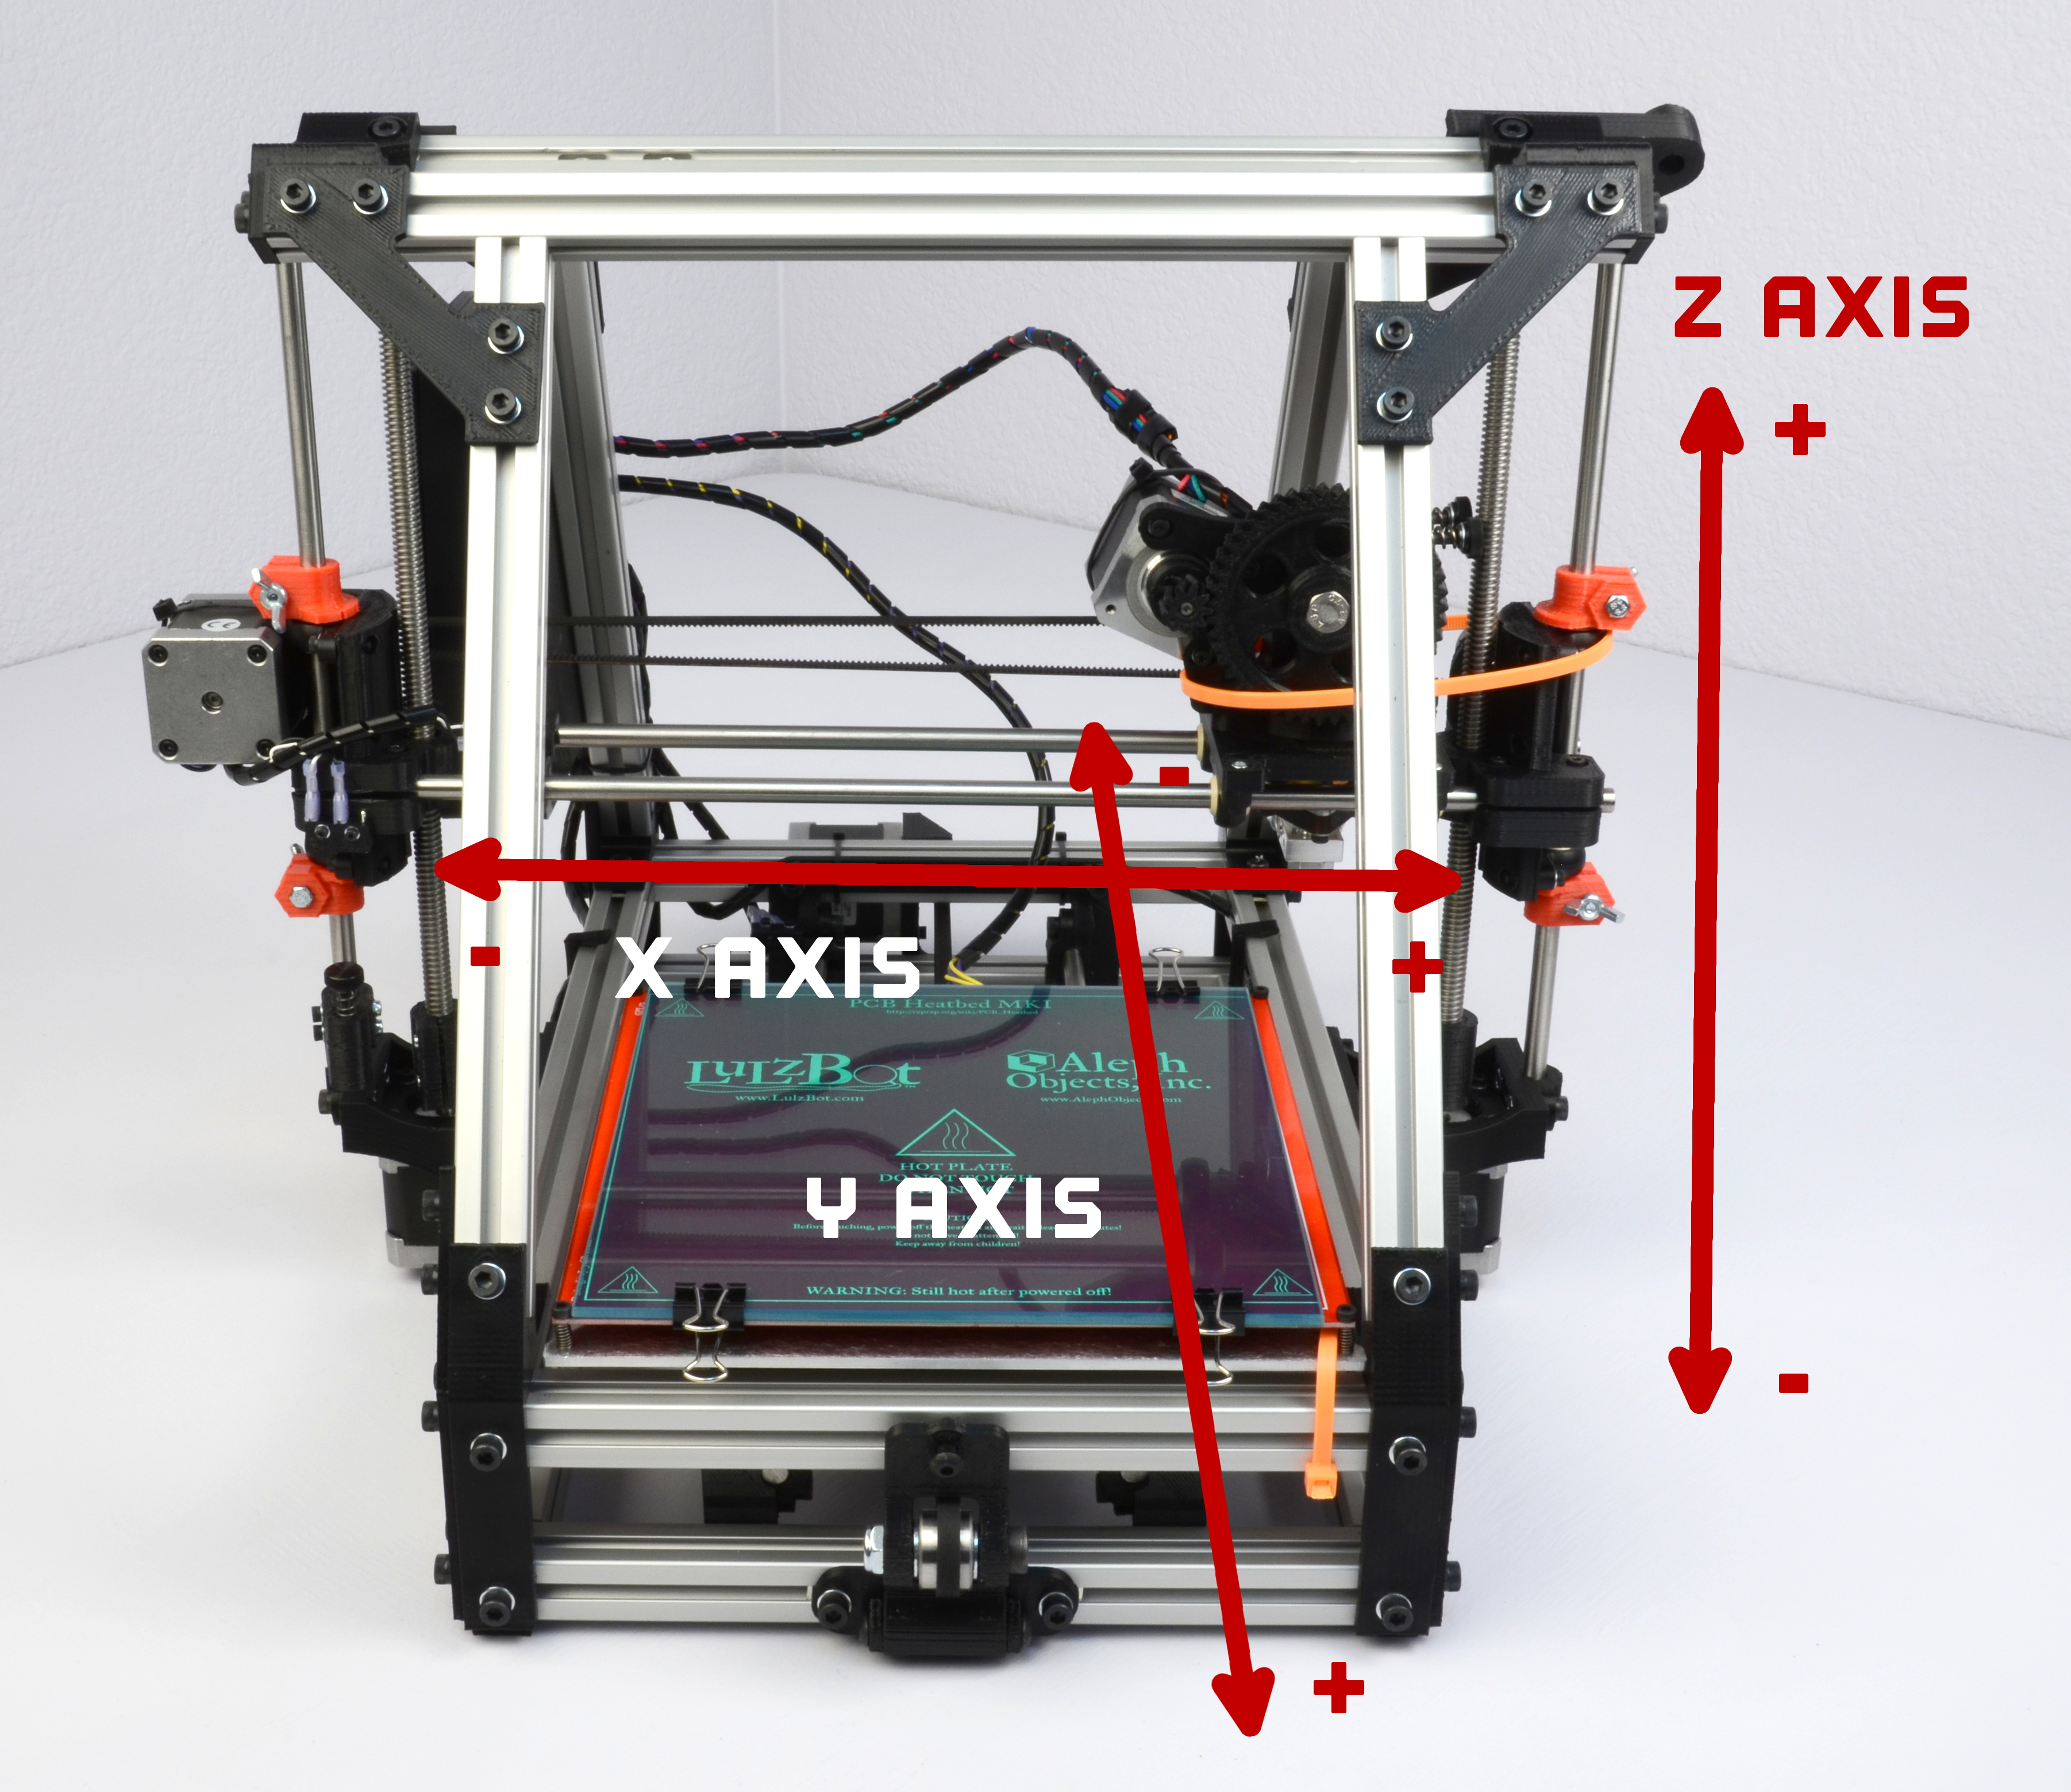
\includegraphics[keepaspectratio=true,angle=0,height=0.4\textheight,width=1.0\textwidth]{axes.jpg}
\caption{Axes movement directions}
\label{fig:axes}
\end{figure}
\begin{figure}[hp]
\centering
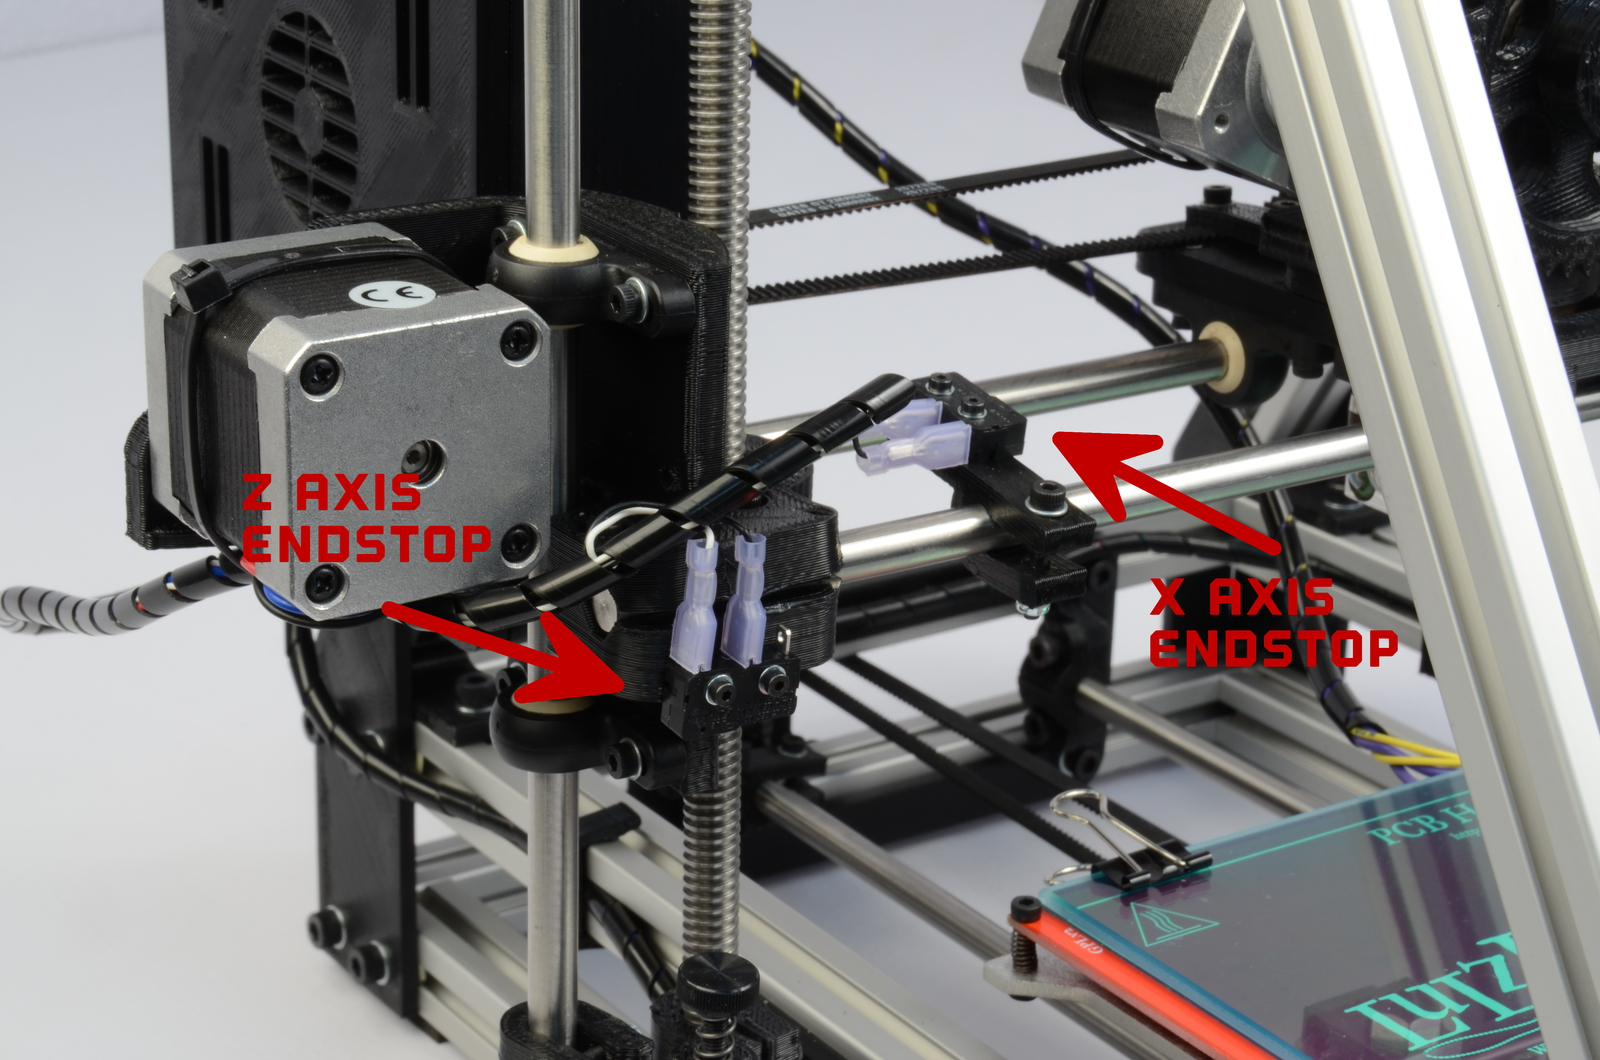
\includegraphics[keepaspectratio=true,angle=0,height=0.4\textheight,width=1.0\textwidth]{xz_endstops.jpg}
\caption{X and Z end stop locations}
\label{fig:xz_endstops}
\end{figure}
\begin{figure}[hp]
\centering
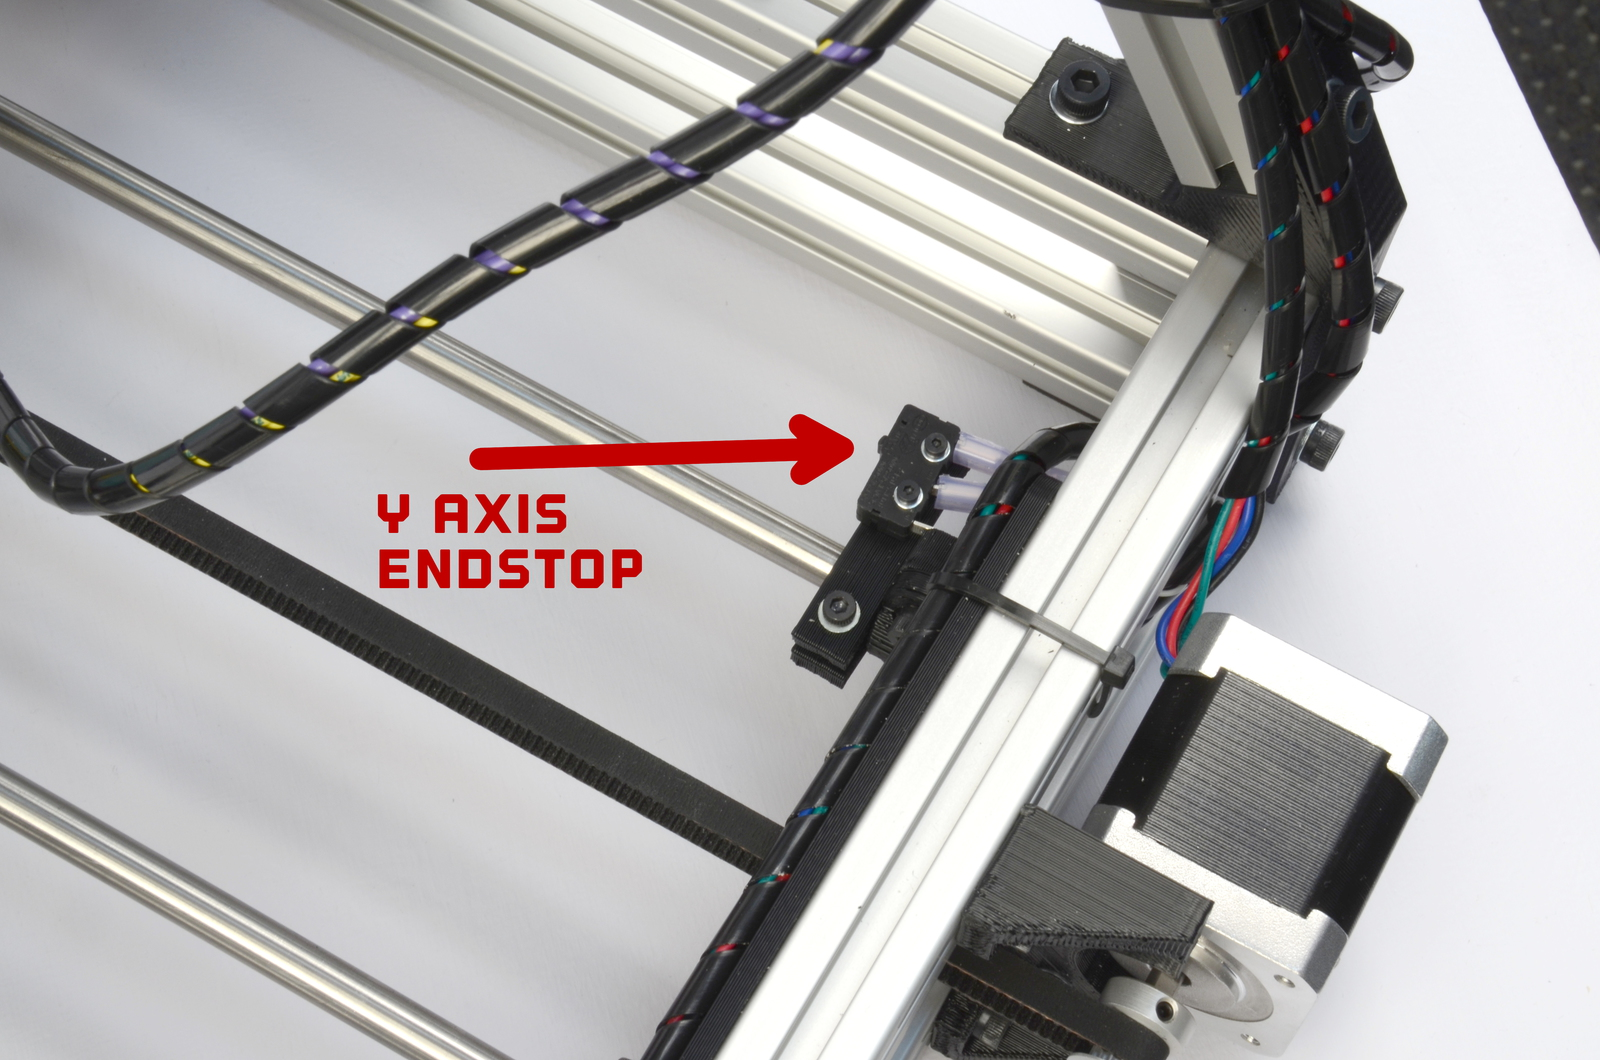
\includegraphics[keepaspectratio=true,angle=0,height=0.4\textheight,width=1.0\textwidth]{y_endstop.jpg}
\caption{Y end stop location}
\label{fig:y_endstop}
\end{figure}

\index{power supply}
\index{USB cable}
\item Unwrap the power supply and USB cable.

\textcolor{red}{MAKE SURE THE POWER SUPPLY IS COMPLETELY UNPLUGGED BEFORE MOVING ON TO THE NEXT STEP}.

\index{electronics receptacles}
\item Locate the power supply and USB receptacles along the bottom of the RAMBo electronics enclosure
(Fig. \ref{fig:electronics_plugs}, page \pageref{fig:electronics_plugs}).
\begin{figure}[hbt]
\centering
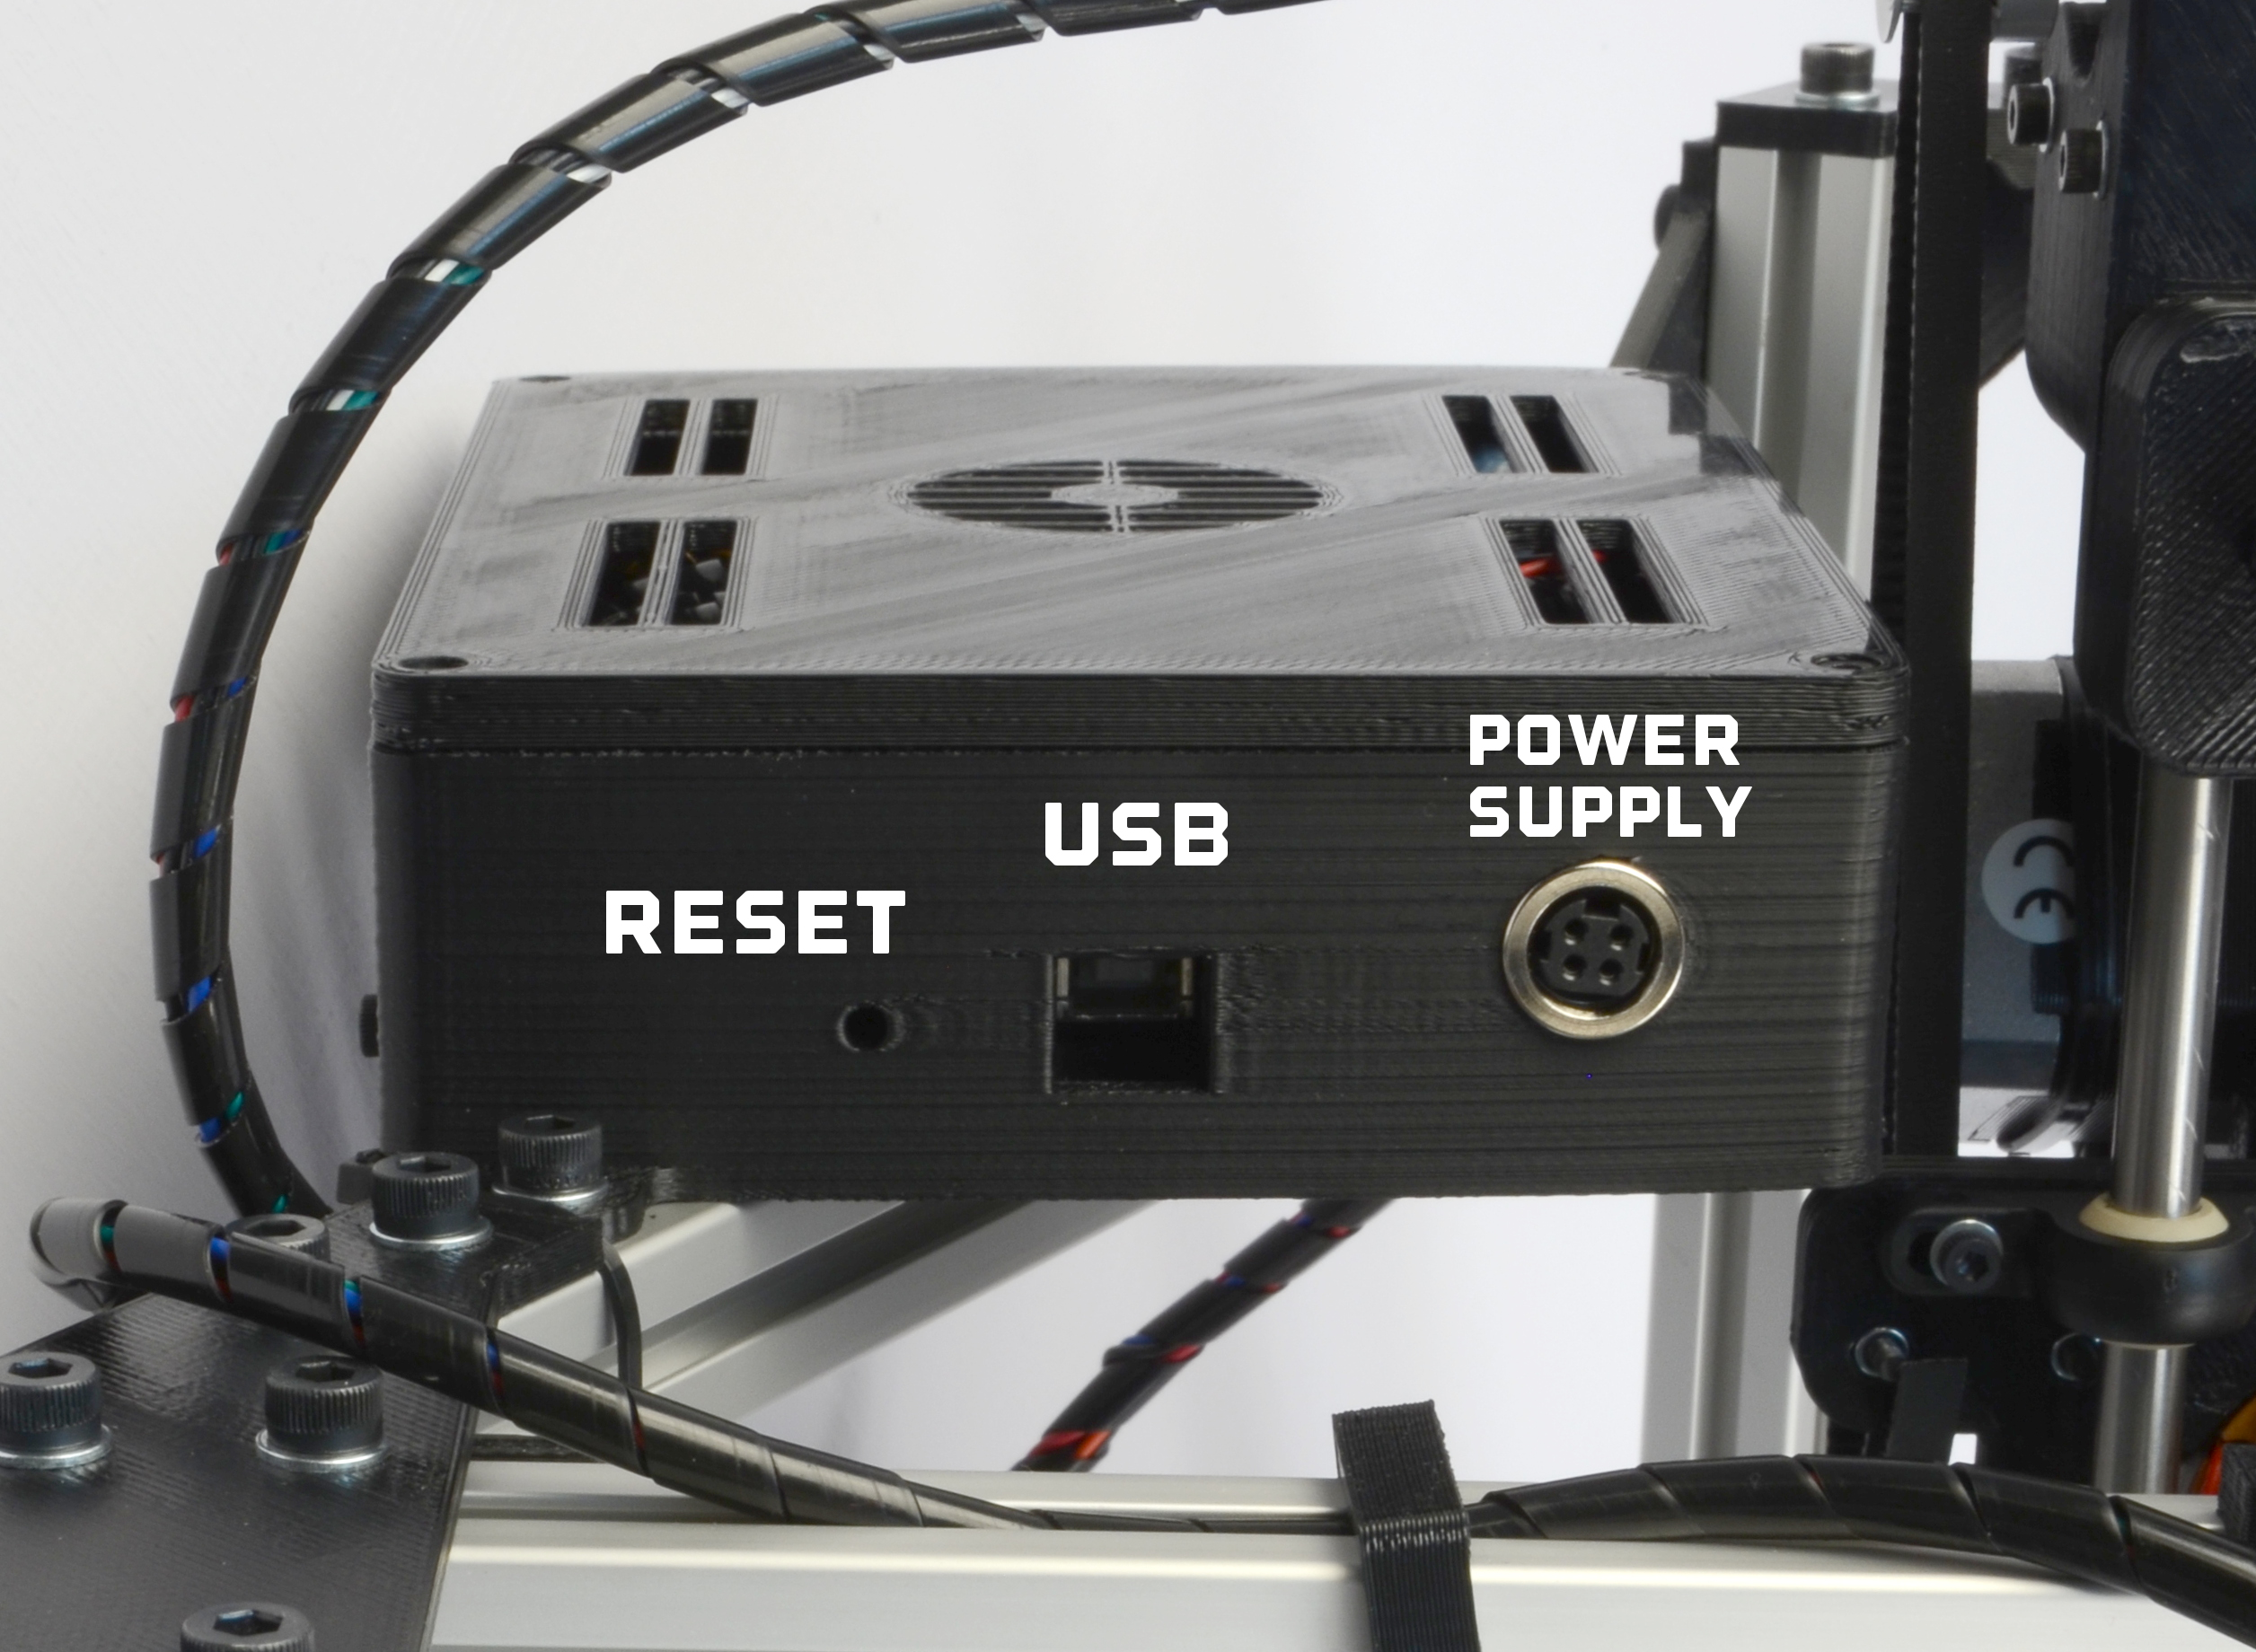
\includegraphics[keepaspectratio=true,angle=0,height=0.4\textheight,width=1.0\textwidth]{electronics_plugs.jpg}
\caption{Power supply and USB receptacles}
\label{fig:electronics_plugs}
\end{figure}
\begin{figure}[hp]
\centering
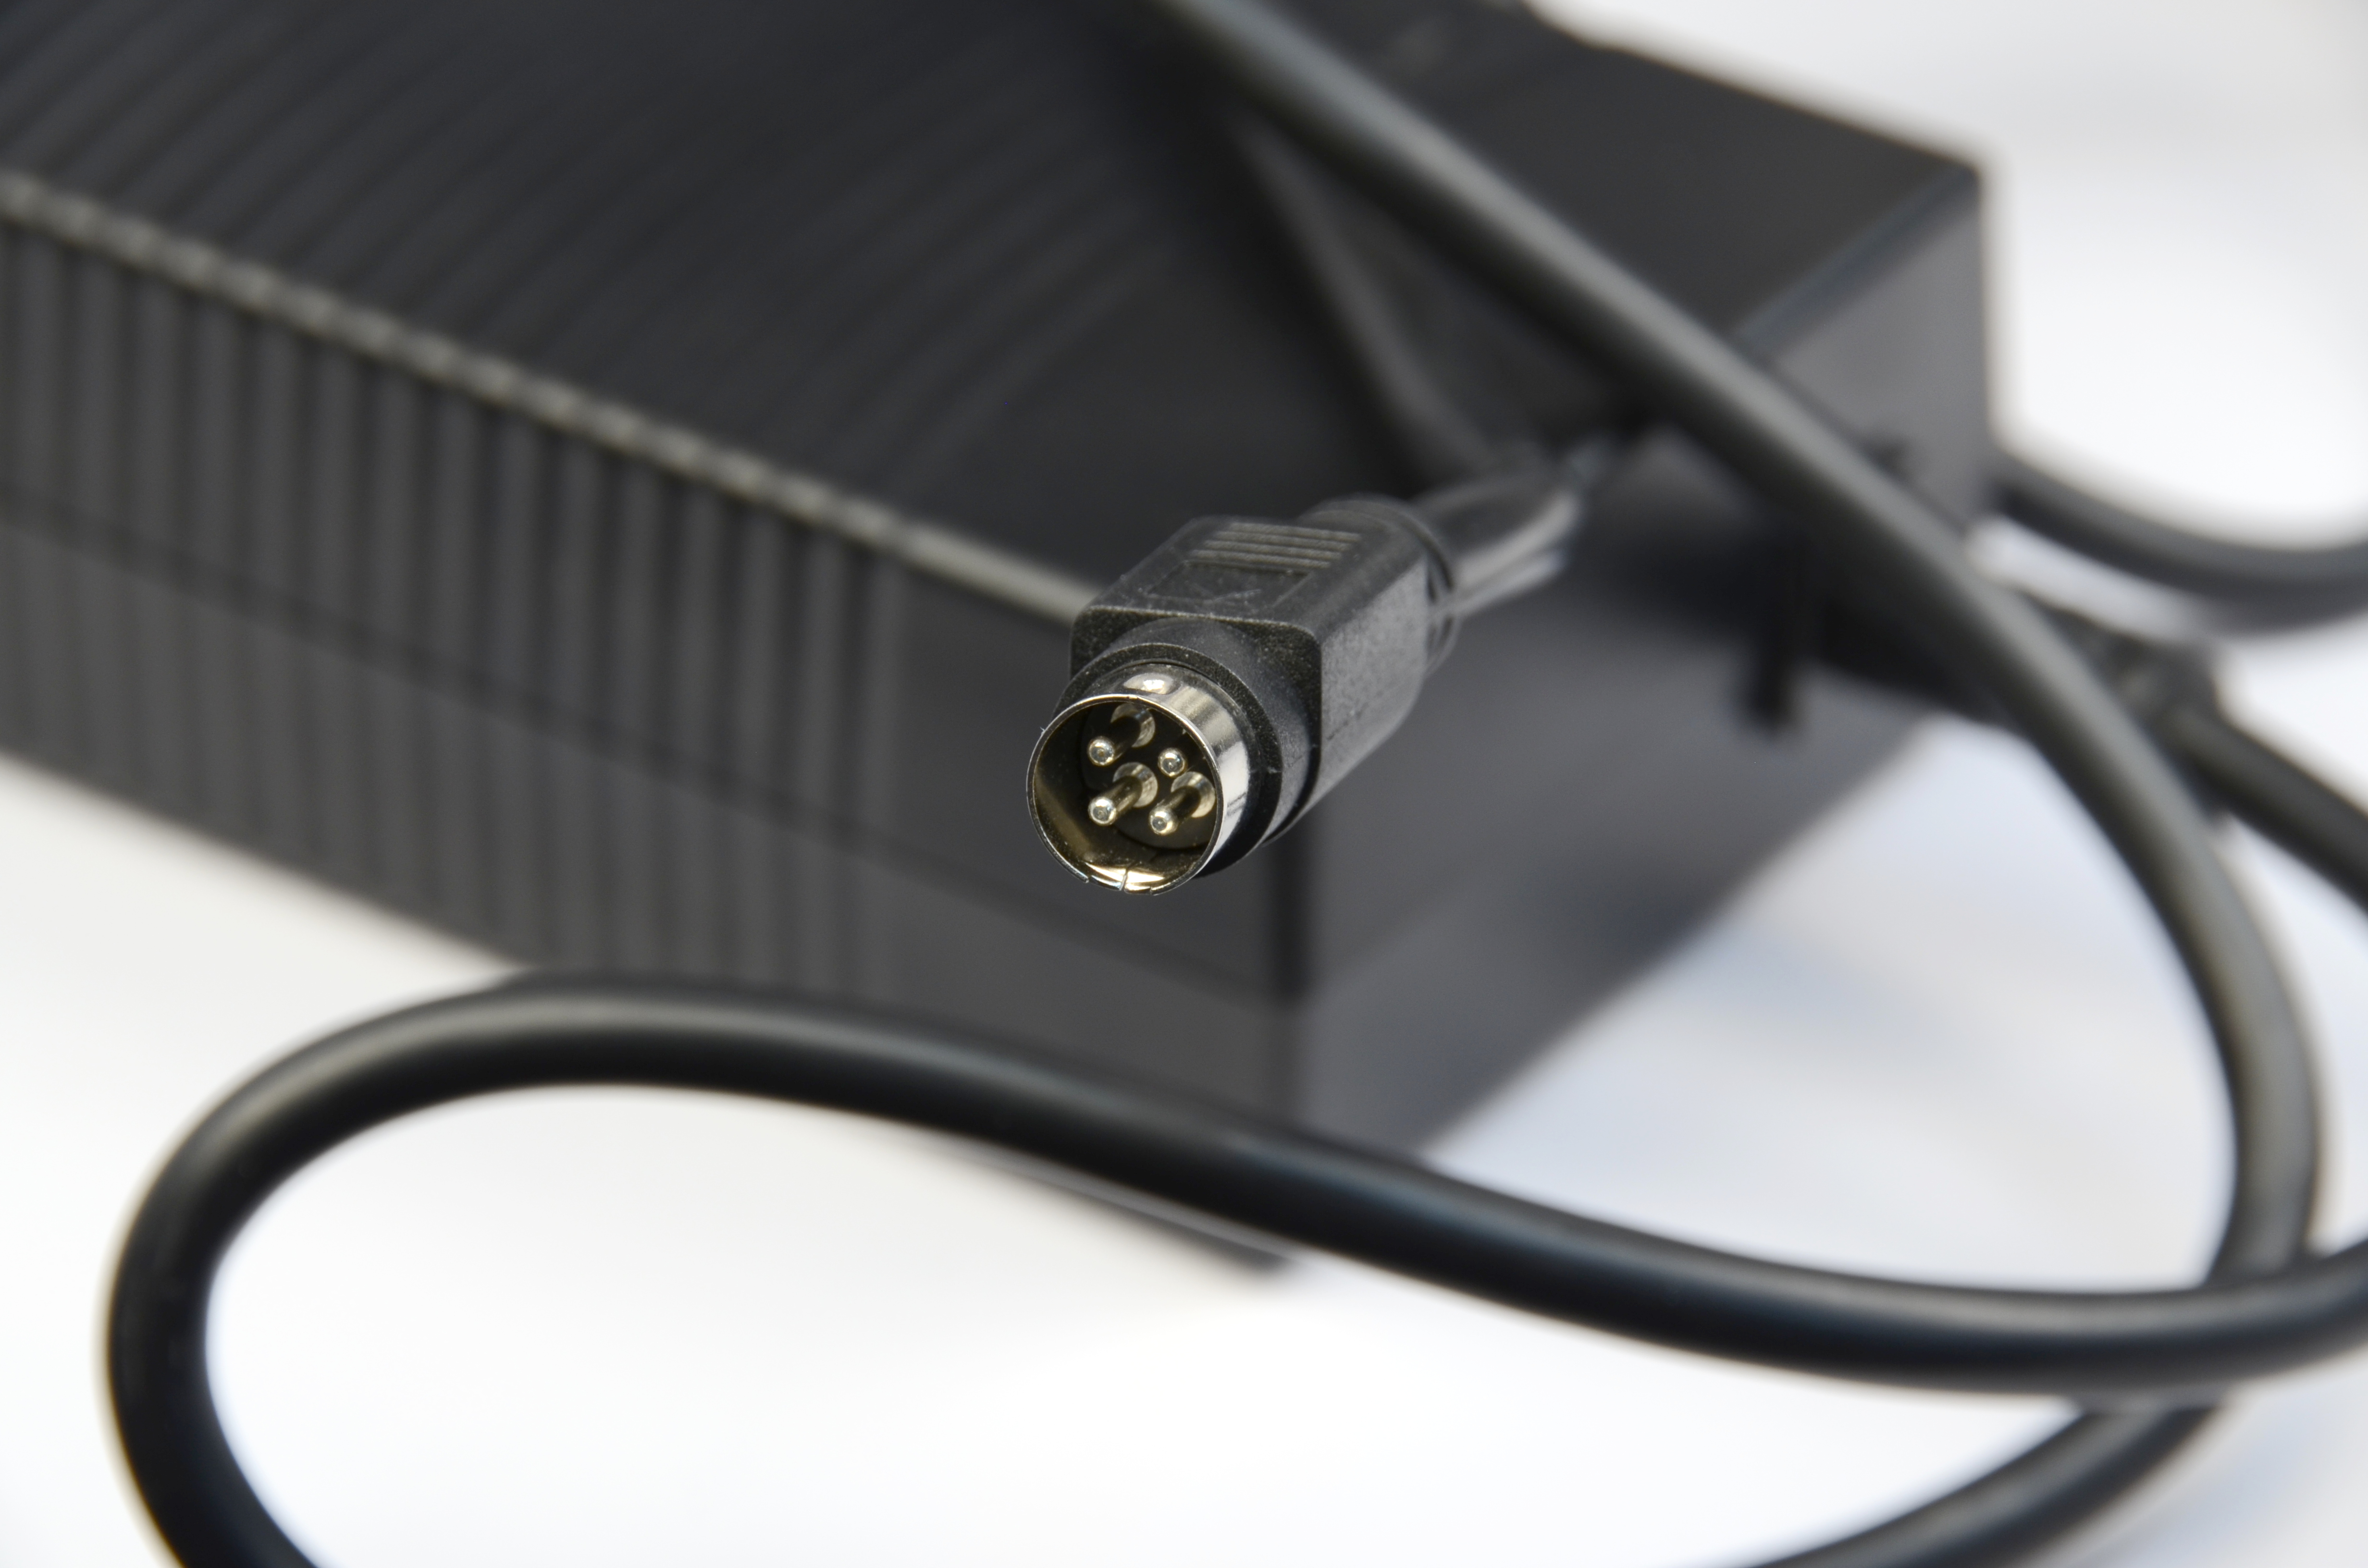
\includegraphics[keepaspectratio=true,angle=0,height=0.4\textheight,width=1.0\textwidth]{ps_plug.jpg}
\caption{Power supply plug}
\label{fig:ps_plug}
\end{figure}
\begin{figure}[hp]
\centering
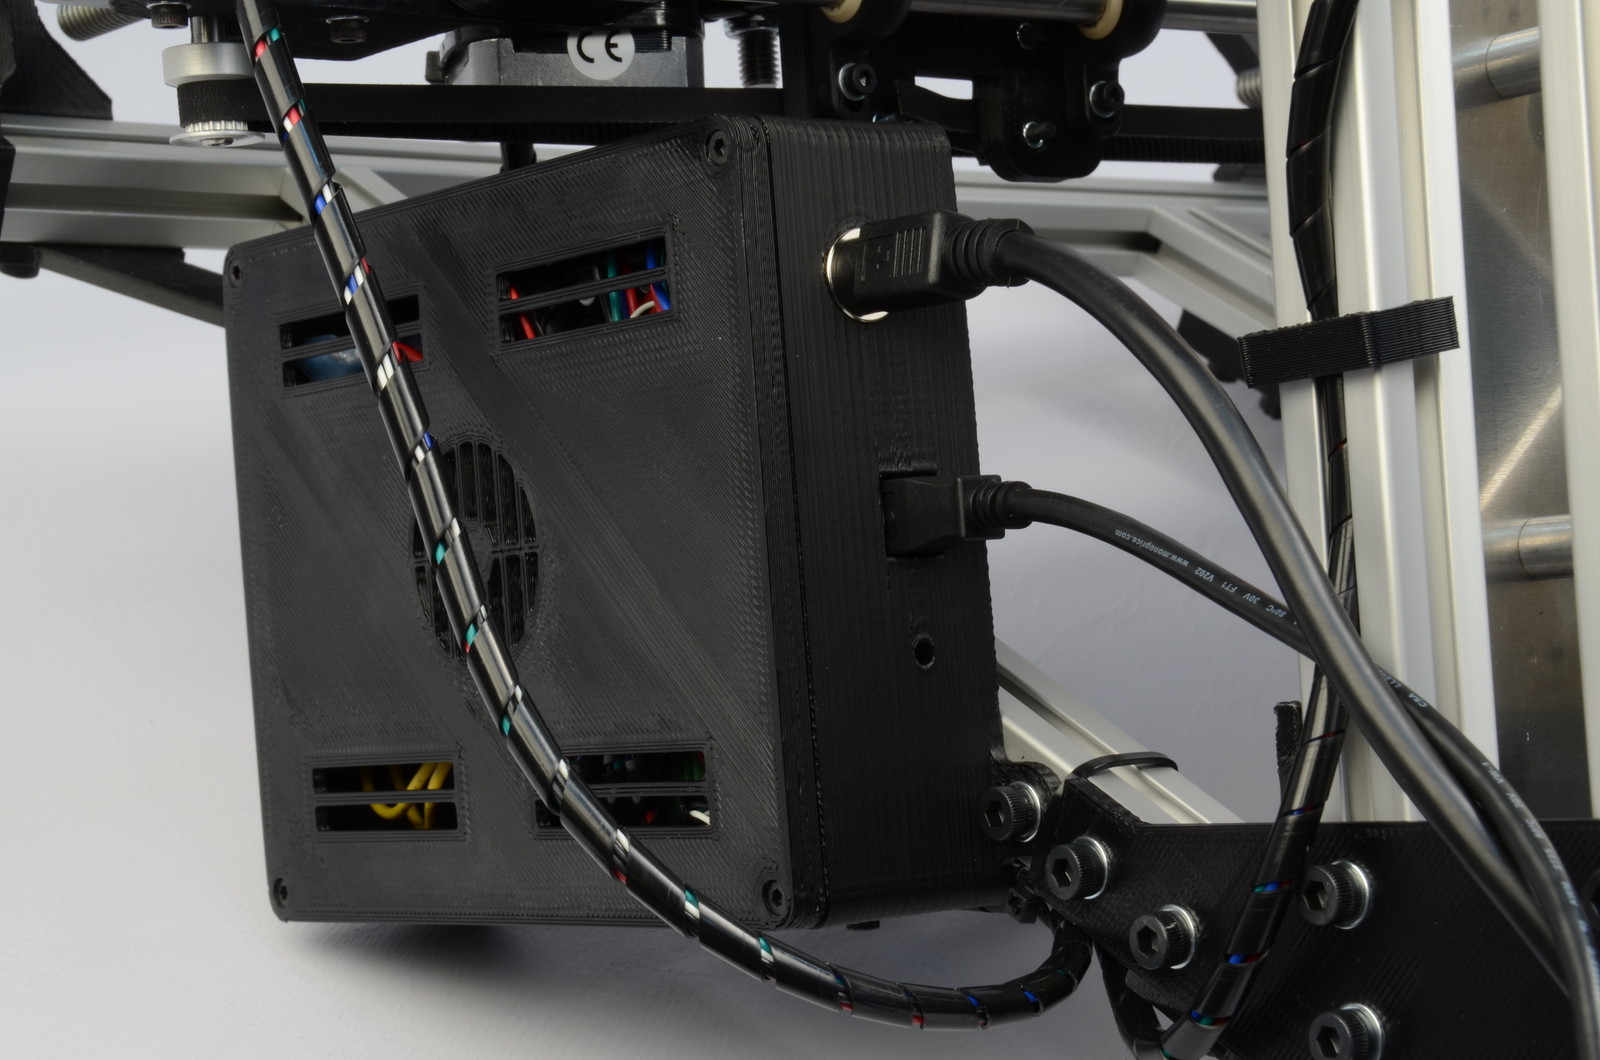
\includegraphics[keepaspectratio=true,angle=0,height=0.4\textheight,width=1.0\textwidth]{electronics_plugs_plugged-in.jpg}
\caption{The power supply and USB plugs correctly plugged in}
\label{fig:electronics_plugs_plugged-in}
\end{figure}

\index{RAMBo}
\item Plug in the USB cable, B plug (square plug) side, into the USB receptacle on the printer electronics. Plug the other end of the USB cable, A plug side, into your computer.

\index{power switch}
\item \textcolor{red}{Make sure the printer power switch is turned off} (the circle side should be depressed). The LED on the power supply should not be lit. Plug in the black power supply plug from the power supply into the power supply receptacle on the printer. The power supply plug must be aligned correctly with the flat side of the plug facing outwards from the printer. (Fig. \ref{fig:ps_plug}, page \pageref{fig:ps_plug}; Fig. \ref{fig:electronics_plugs_plugged-in}, page \pageref{fig:electronics_plugs_plugged-in}). Now you can plug in the AC power plug from the power supply into an AC power outlet.

\index{spool}
\item Locate the plastic filament spool
(Fig. \ref{fig:spool}, page \pageref{fig:spool}).
\begin{figure}[hbt]
\centering
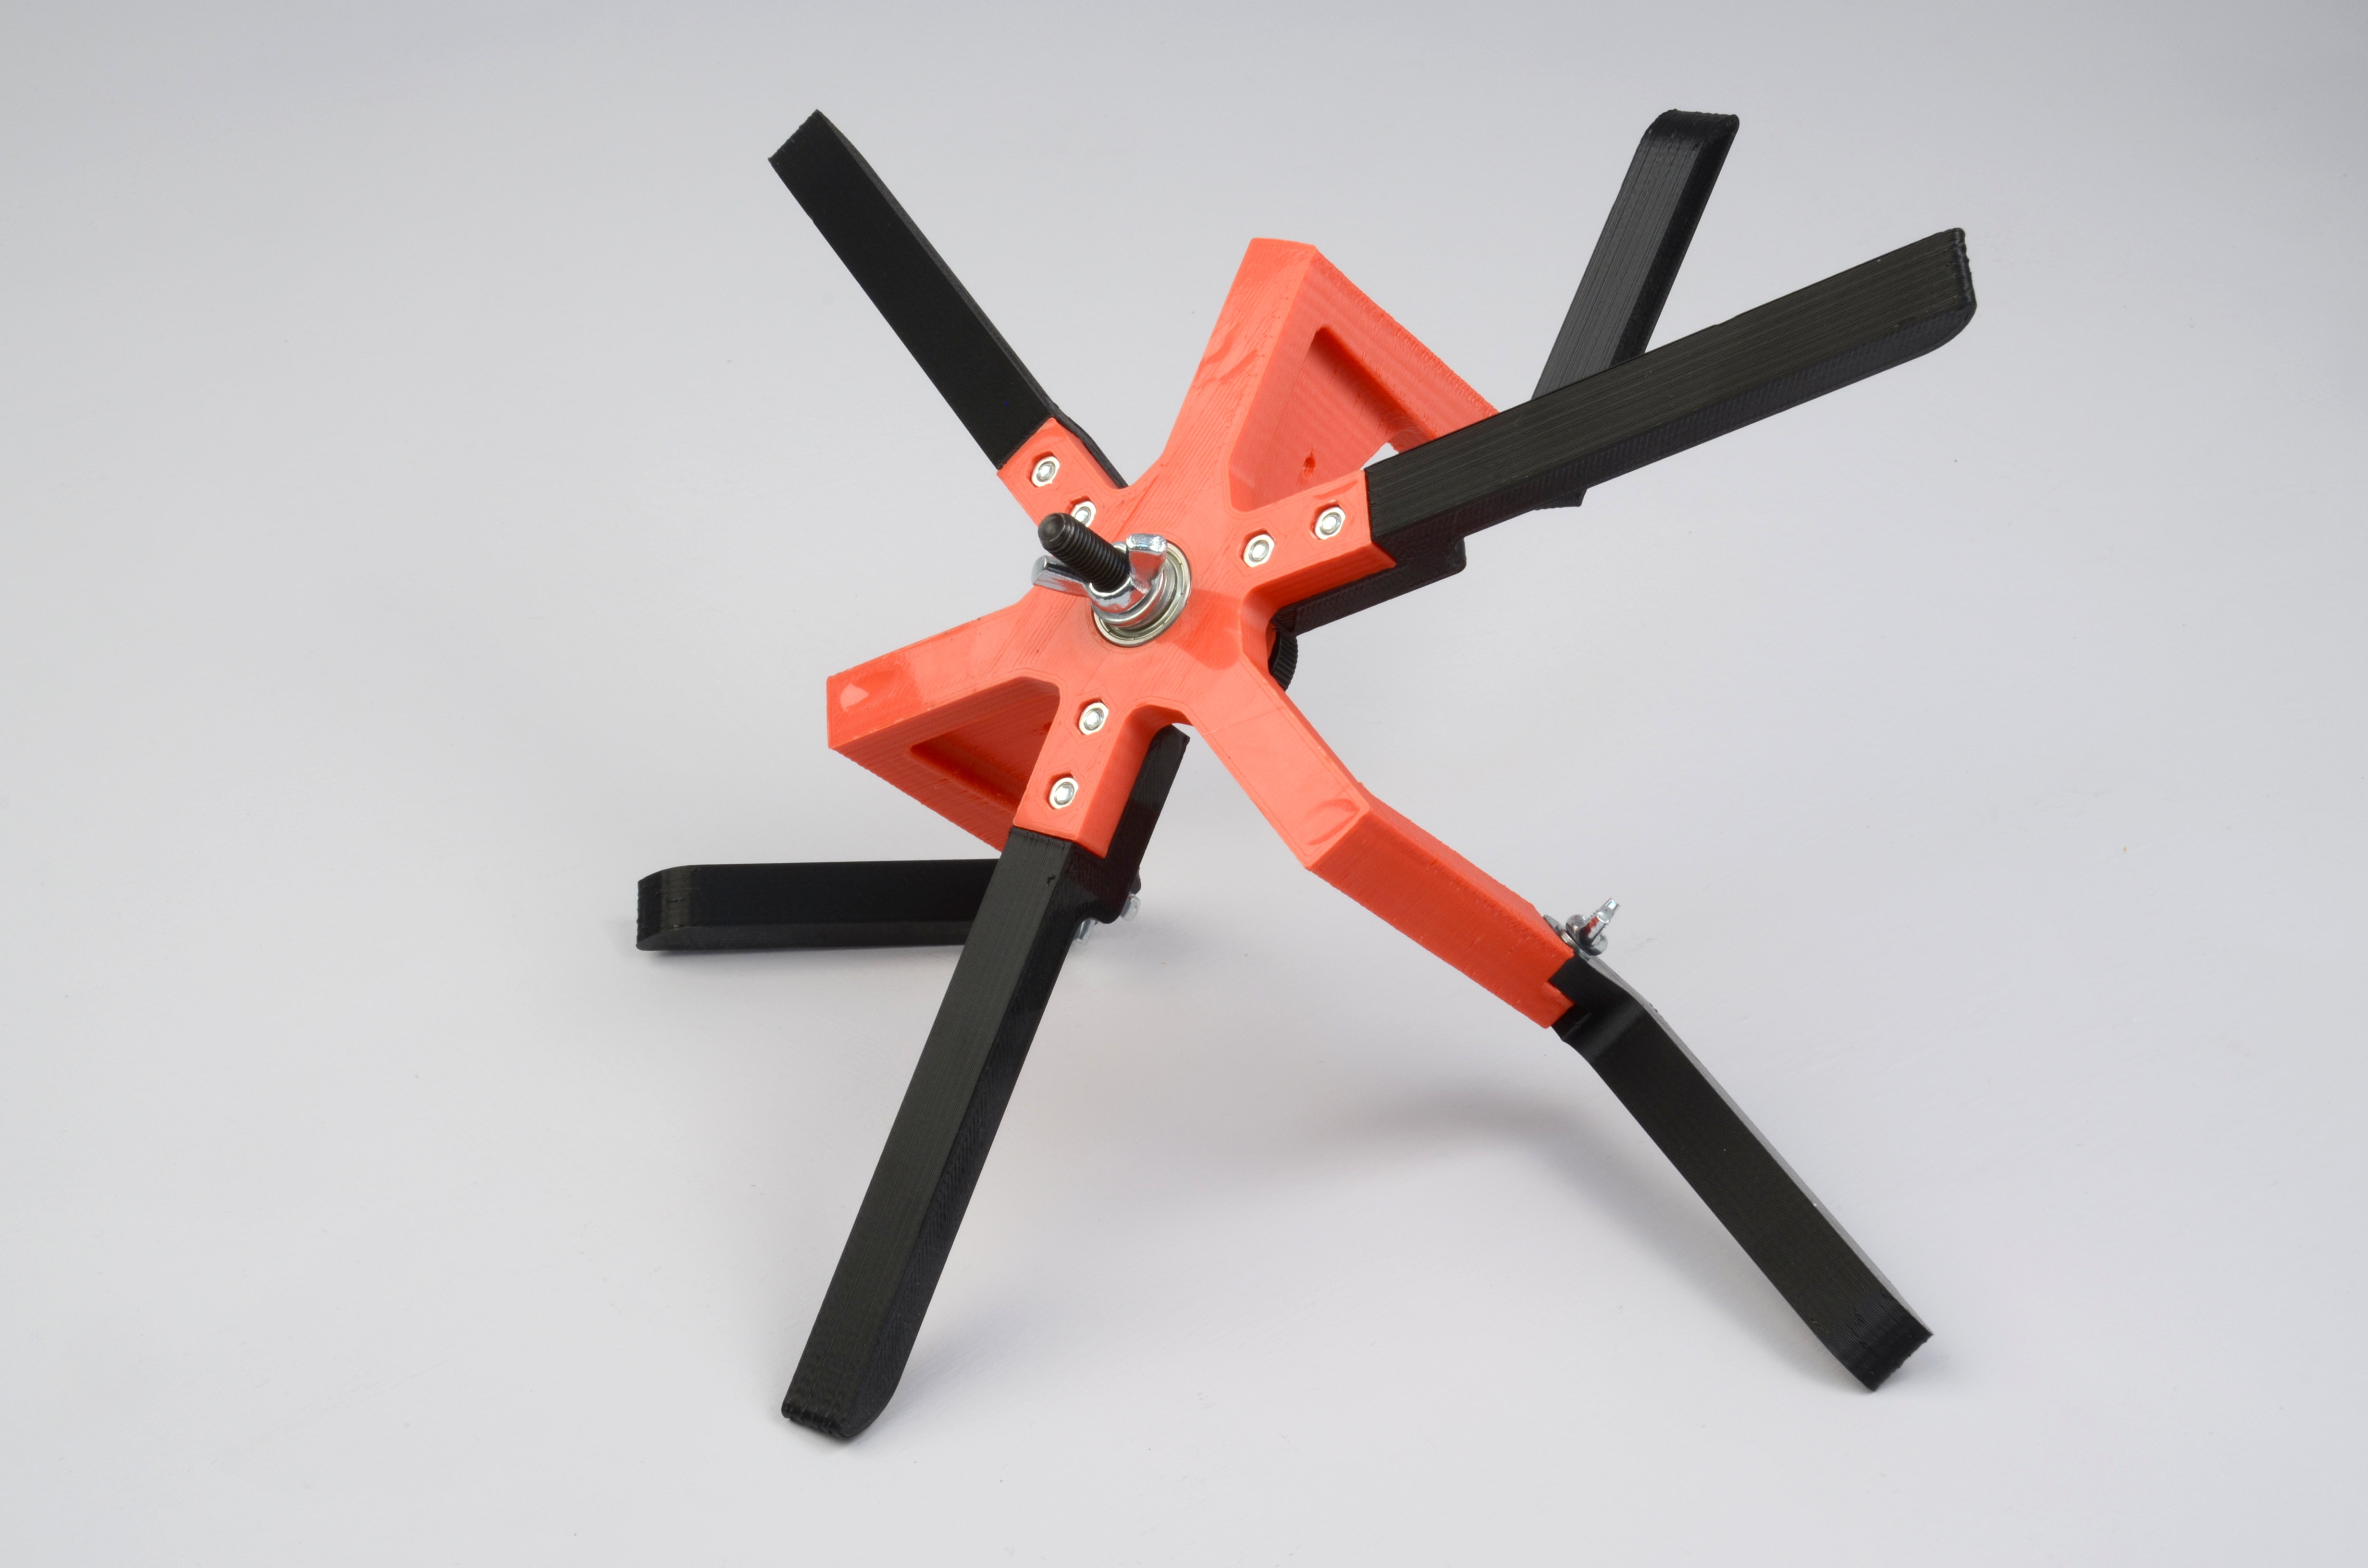
\includegraphics[keepaspectratio=true,angle=0,height=0.4\textheight,width=1.0\textwidth]{spool.jpg}
\caption{Spool}
\label{fig:spool}
\end{figure}

\index{wrench}
\index{pliers}
\item Remove the large wing nut from the back of the spool. Take off one washer leaving the other two on the spool mounting bolt. Now locate the spool mount arm on the top right facing the rear of the printer
(Fig. \ref{fig:spool_mount}, page \pageref{fig:spool_mount}).
\begin{figure}[hbt]
\centering
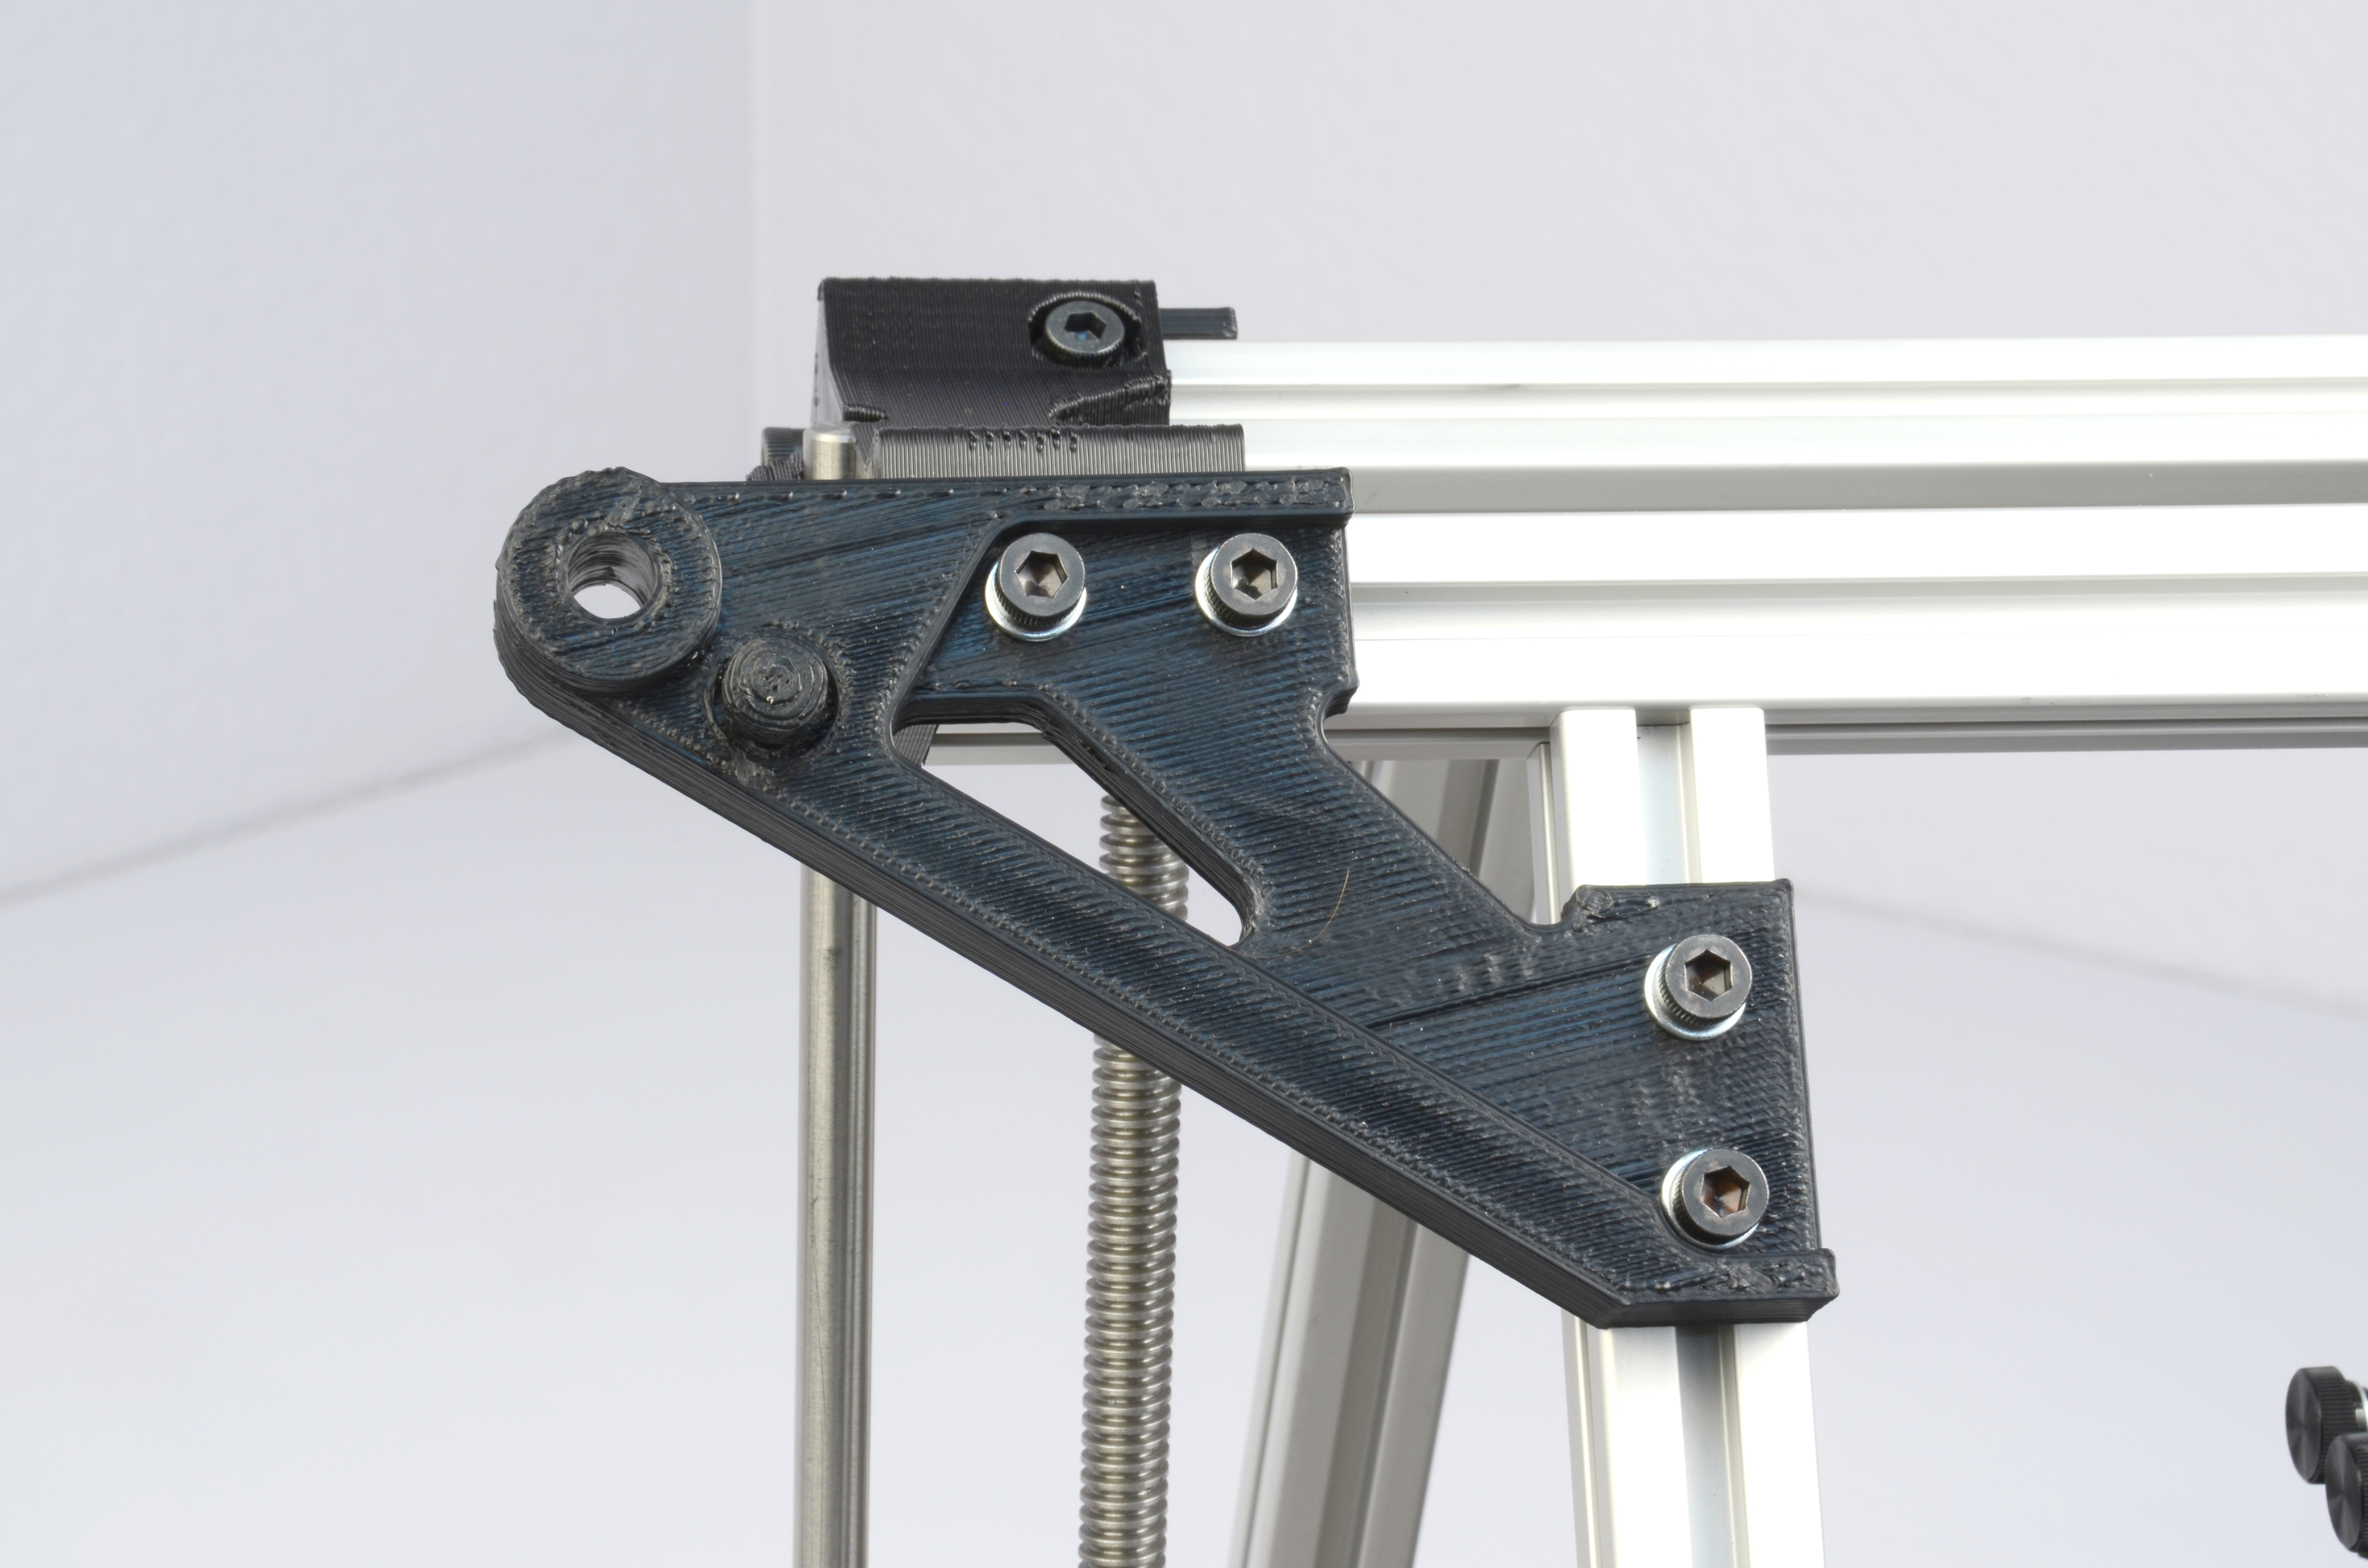
\includegraphics[keepaspectratio=true,angle=0,height=0.4\textheight,width=1.0\textwidth]{spool_mount.jpg}
\caption{Spool mount}
\label{fig:spool_mount}
\end{figure}
Slide the spool mounting bolt through the hole in the spool mount arm. From the back of the spool mount arm slide the one washer on to the spool mounting bolt and turn on and snug tighten the wing nut
(Fig. \ref{fig:spool_mounted}, page \pageref{fig:spool_mounted}).
\begin{figure}[hbt]
\centering
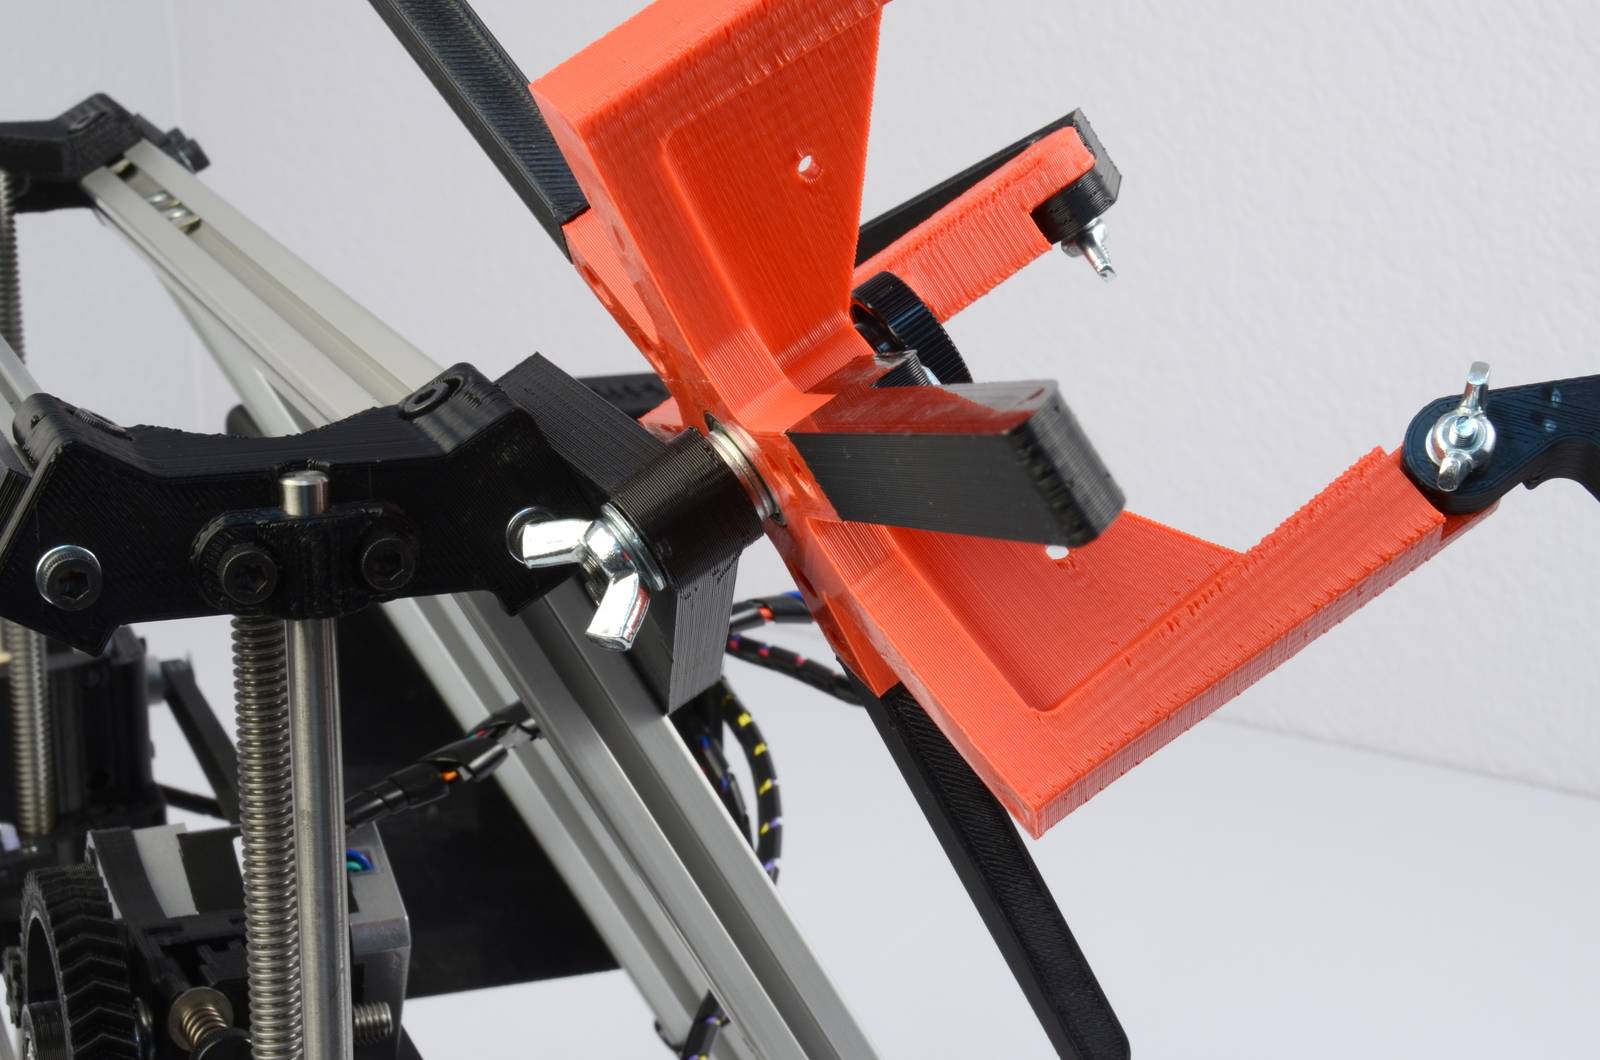
\includegraphics[keepaspectratio=true,angle=0,height=0.4\textheight,width=1.0\textwidth]{spool_mounted.jpg}
\caption{Spool mounted}
\label{fig:spool_mounted}
\end{figure}

\index{PTFE tube}
\item Locate the filament guide with attached PTFE tube
(Fig. \ref{fig:filament_guide}, page \pageref{fig:filament_guide}).
\begin{figure}[hbt]
\centering
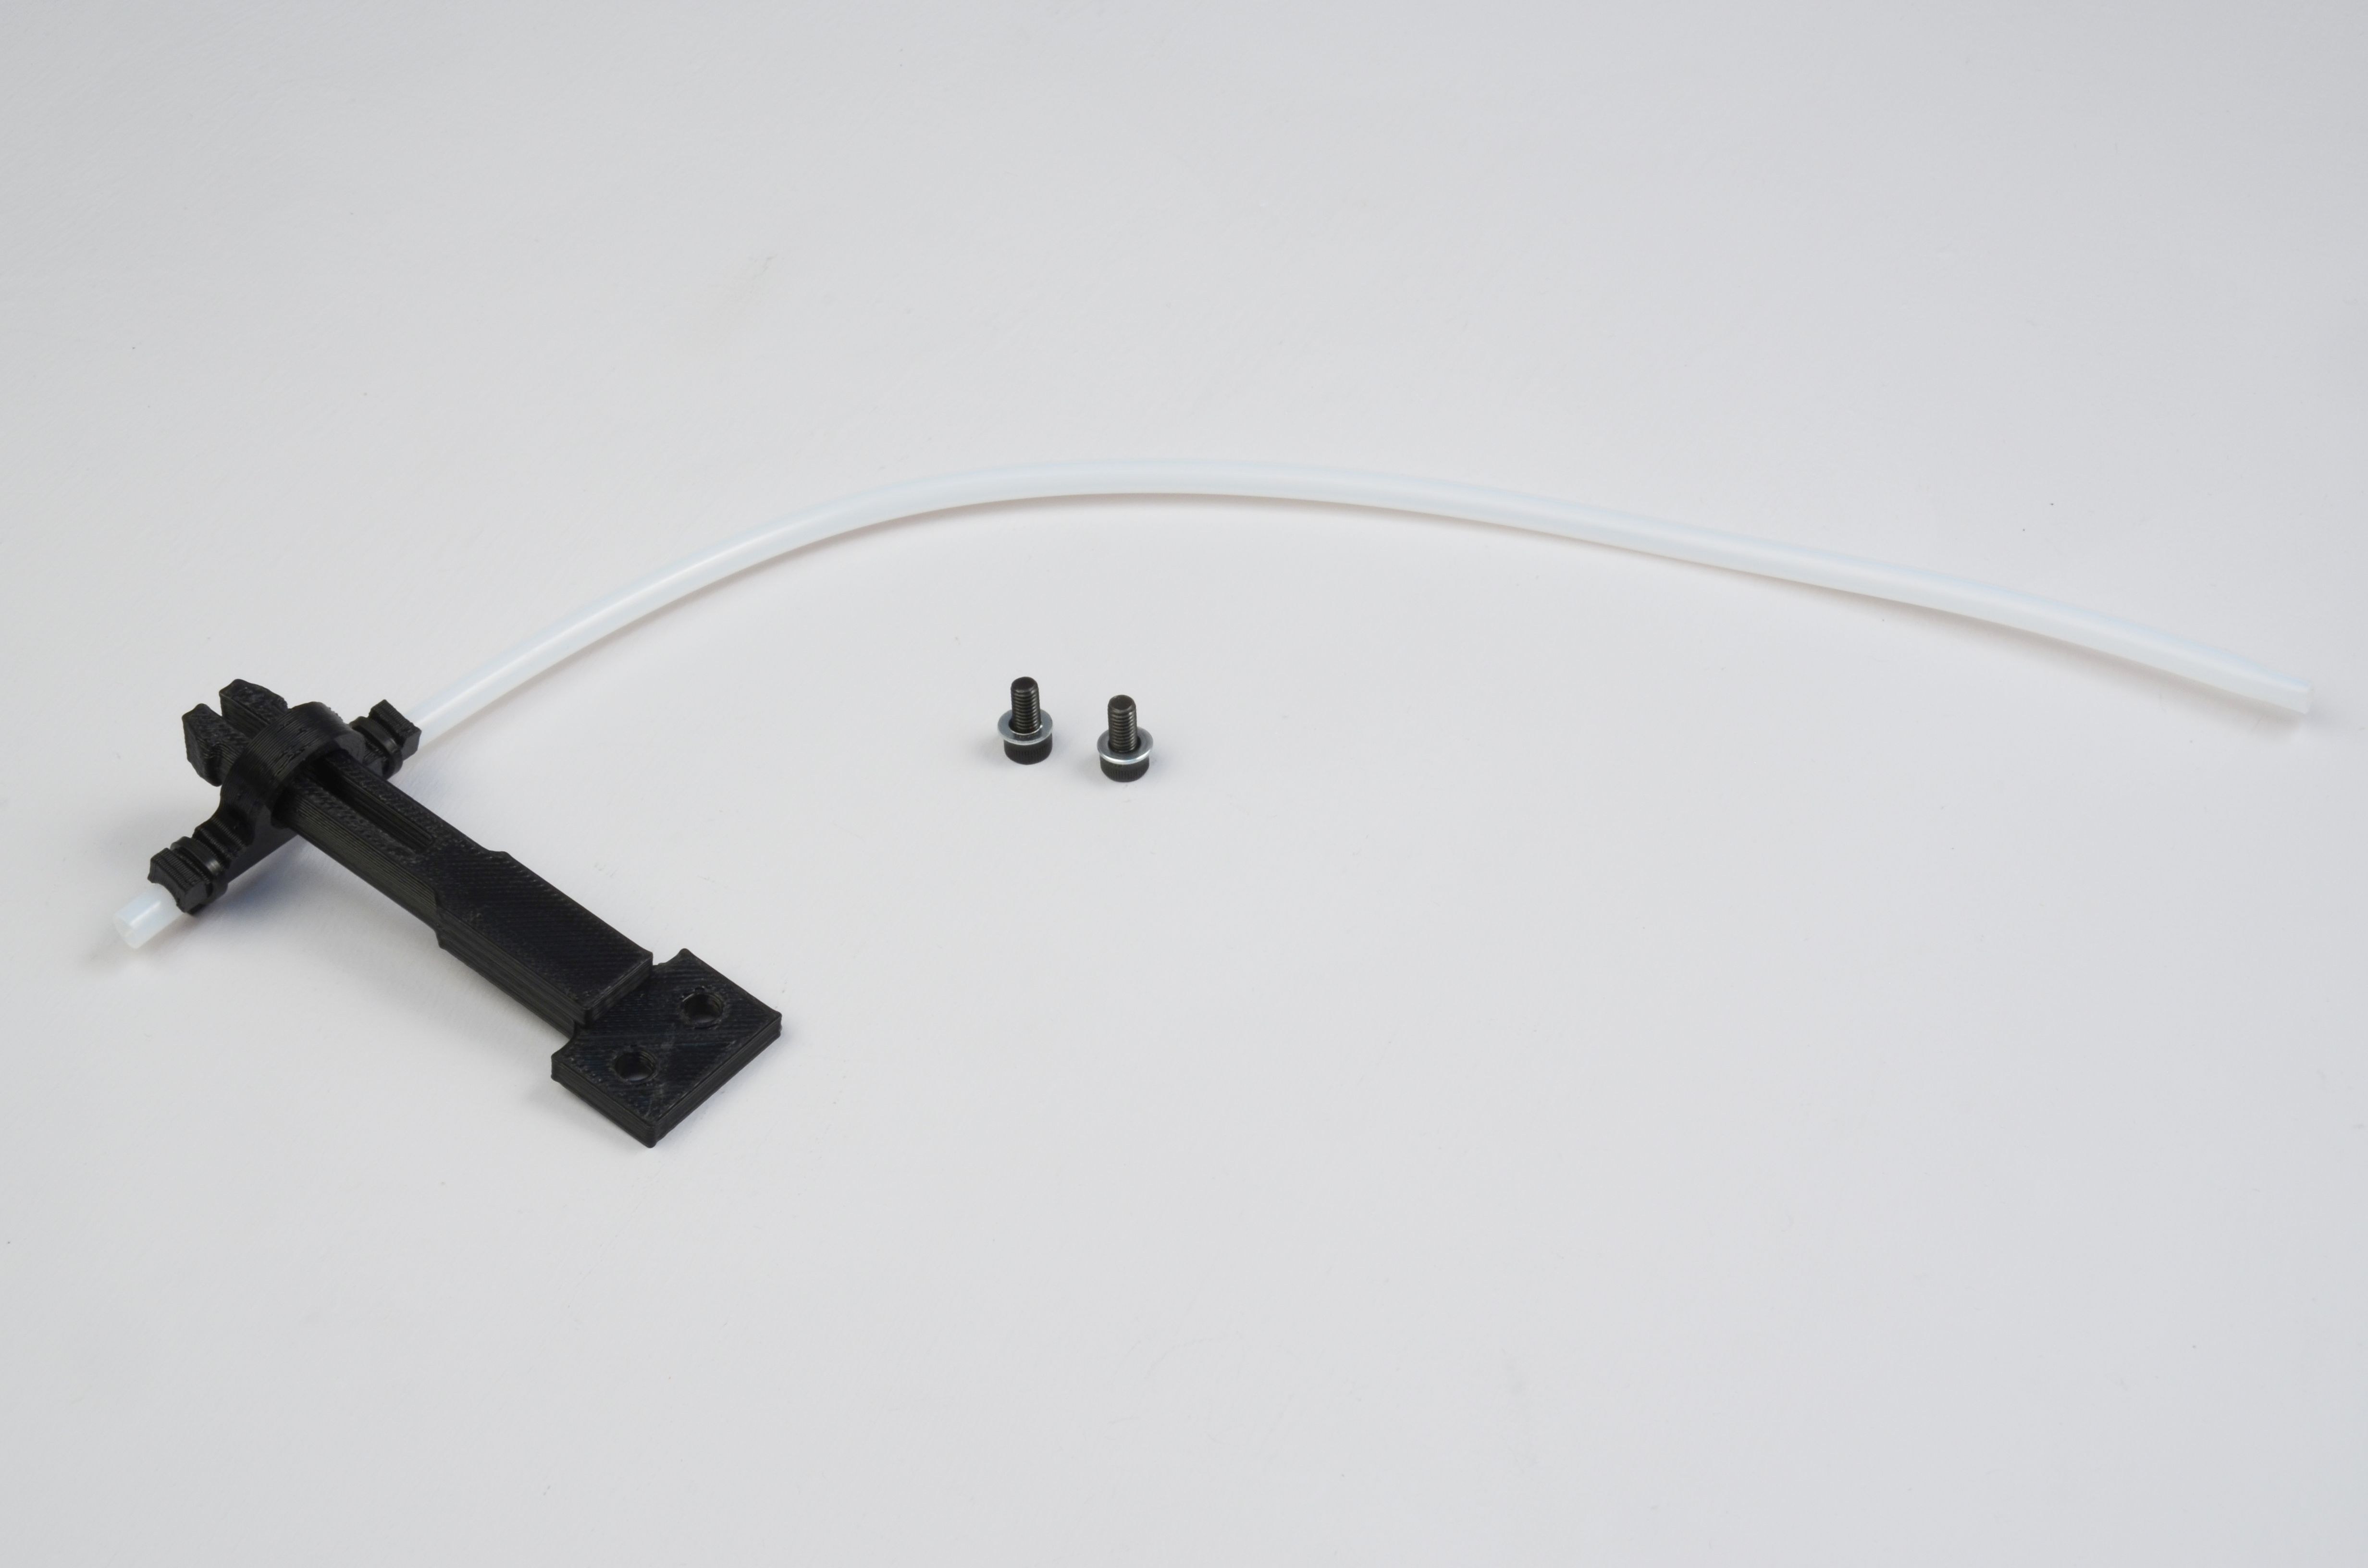
\includegraphics[keepaspectratio=true,angle=0,height=0.4\textheight,width=1.0\textwidth]{filament_guide.jpg}
\caption{Filament Guide}
\label{fig:filament_guide}
\end{figure}

Locate the top most horizontal aluminum extrusion closest to the filament spool
(Fig. \ref{fig:filament_guide_nuts}, page \pageref{fig:filament_guide_nuts}).
\begin{figure}[hbt]
\centering
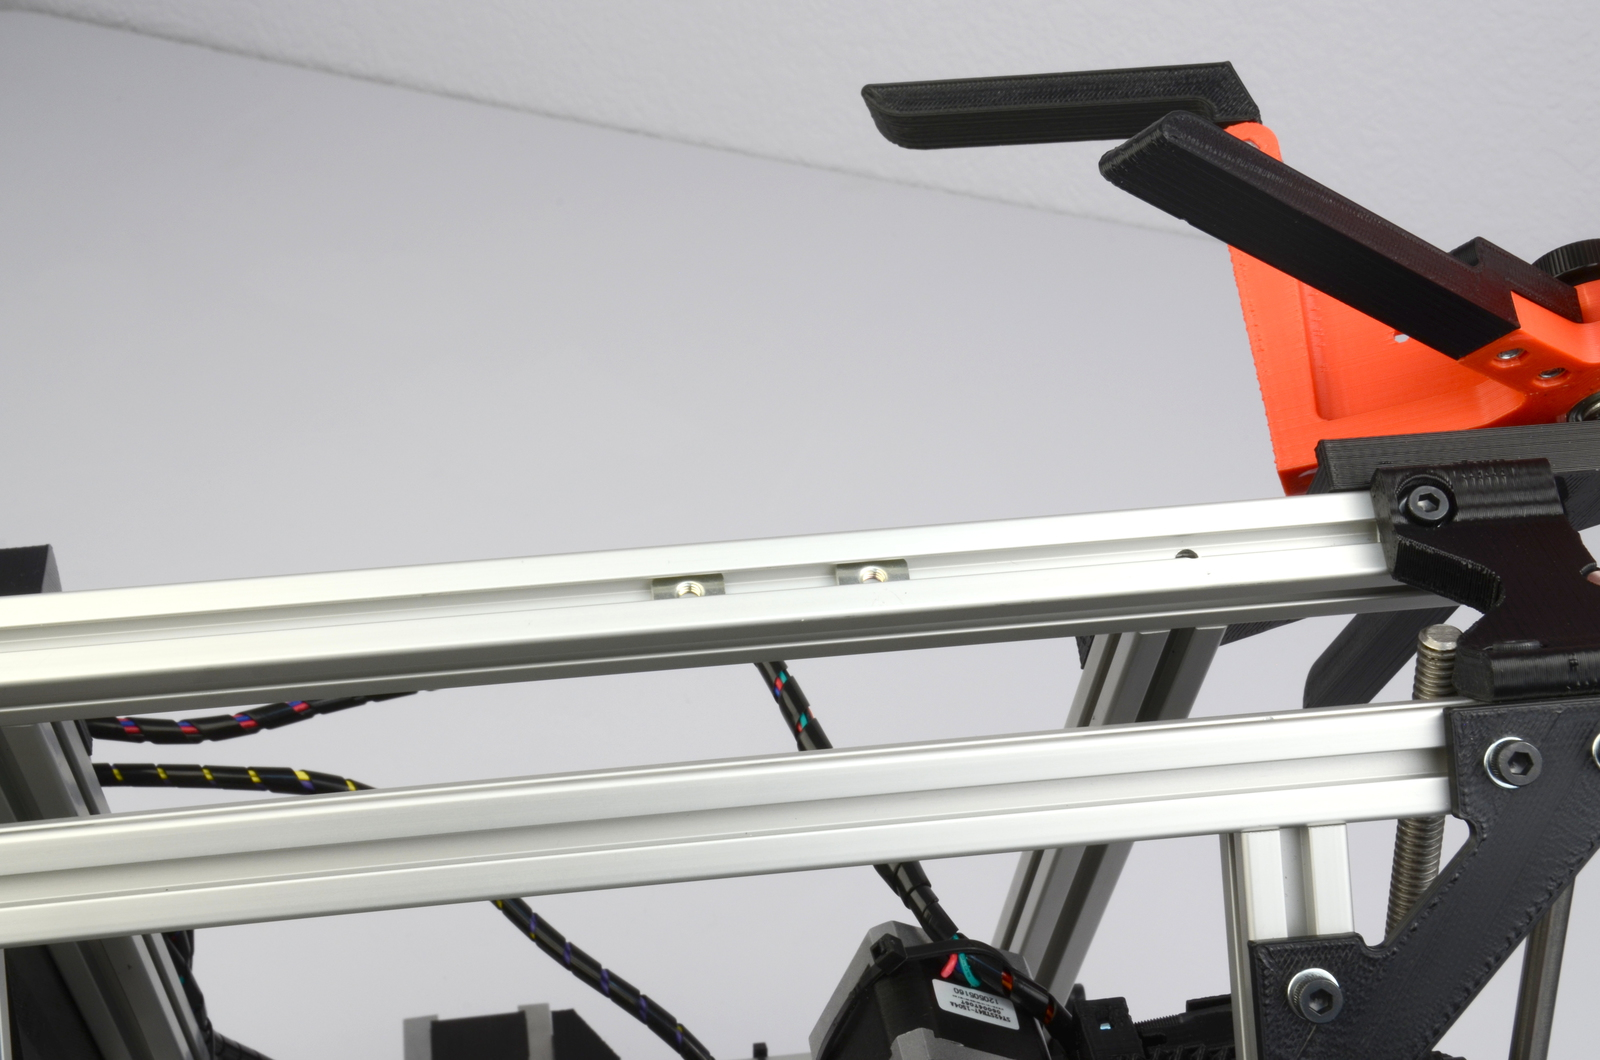
\includegraphics[keepaspectratio=true,angle=0,height=0.4\textheight,width=1.0\textwidth]{filament_guide_nuts.jpg}
\caption{Filament Guide Nuts}
\label{fig:filament_guide_nuts}
\end{figure}

In the extrusion you will find two loose t-slot nuts. The filament guide attaches to the printer by screwing in the two bolts through the filament guide into the t-slot nuts. First thread the two bolts through the filament guide into the t-slot nuts. Leave the bolts loose enough so the filament guide can slide back and forth across the extrusion. Set the filament guide 1.5-2cm away from the end of the lower arms of the filament spool
(Fig. \ref{fig:filament_guide_setting}, page \pageref{fig:filament_guide_setting}).
\begin{figure}[hbt]
\centering
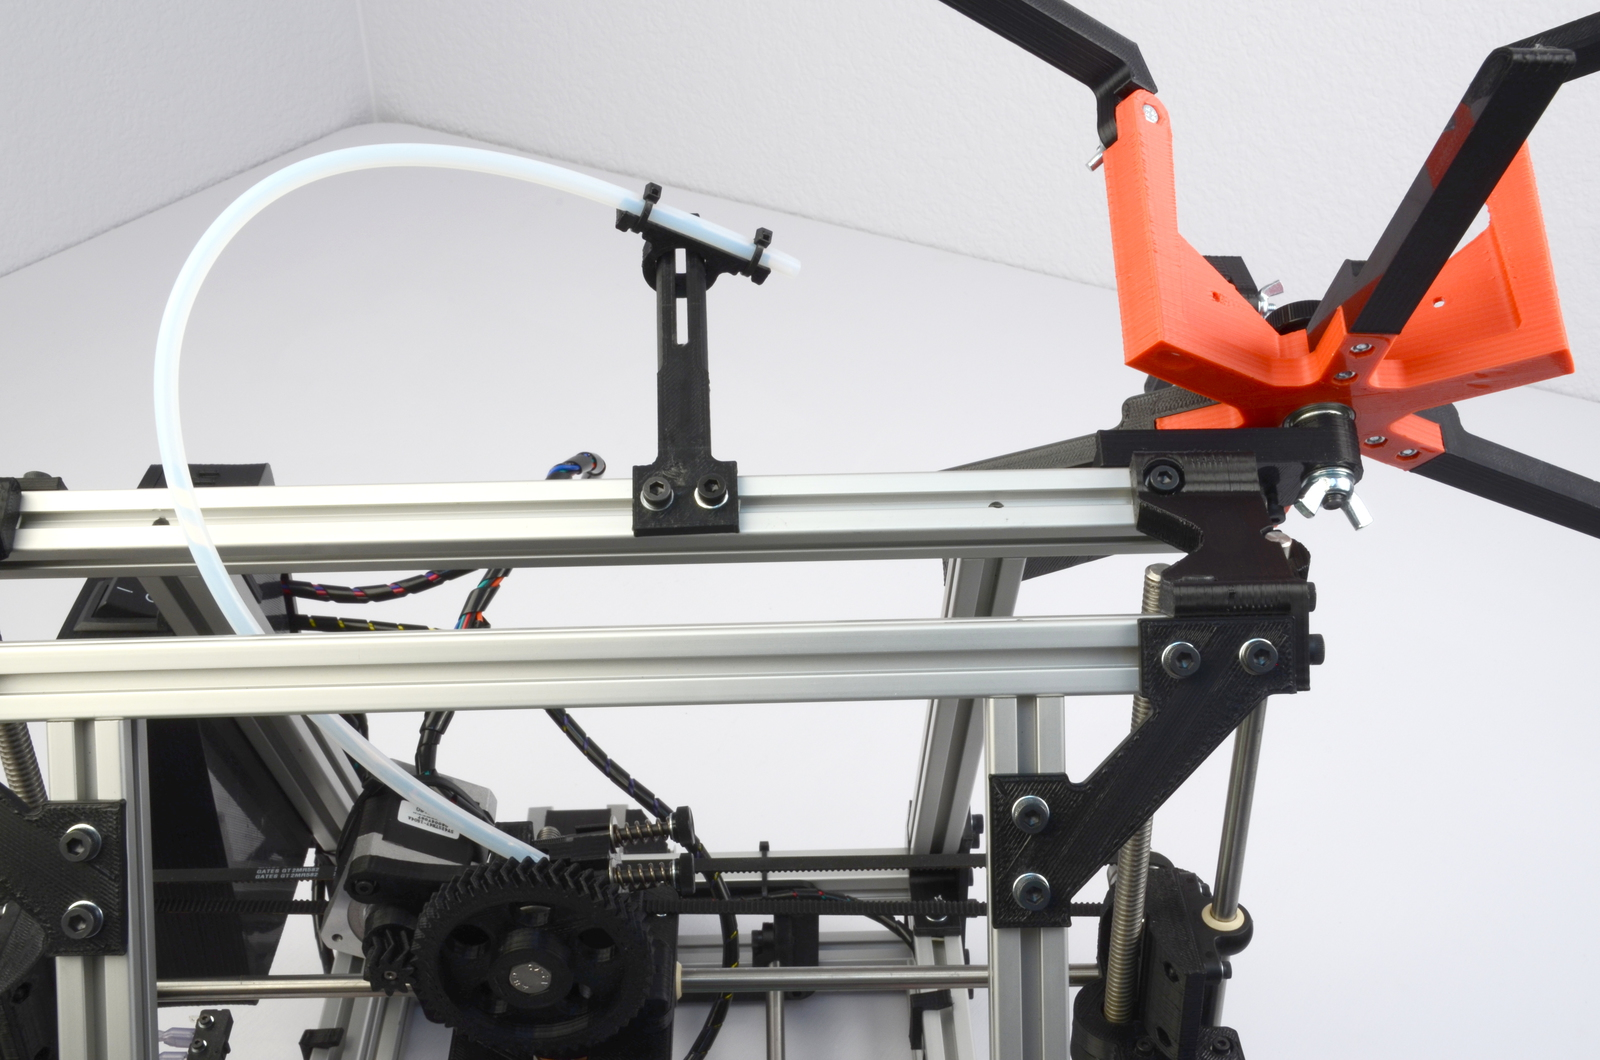
\includegraphics[keepaspectratio=true,angle=0,height=0.4\textheight,width=1.0\textwidth]{filament_guide_setting.jpg}
\caption{Filament Guide Setting}
\label{fig:filament_guide_setting}
\end{figure}
Once the filament guide is set in place, tighten down the two bolts.

\item Insert the micro SD card into the micro SD card slot, found on the top of the RAMBo electronics enclosure, shown in
Figure \ref{fig:sdramps}, page \pageref{fig:sdramps}.
\begin{figure}[hbt]
\centering
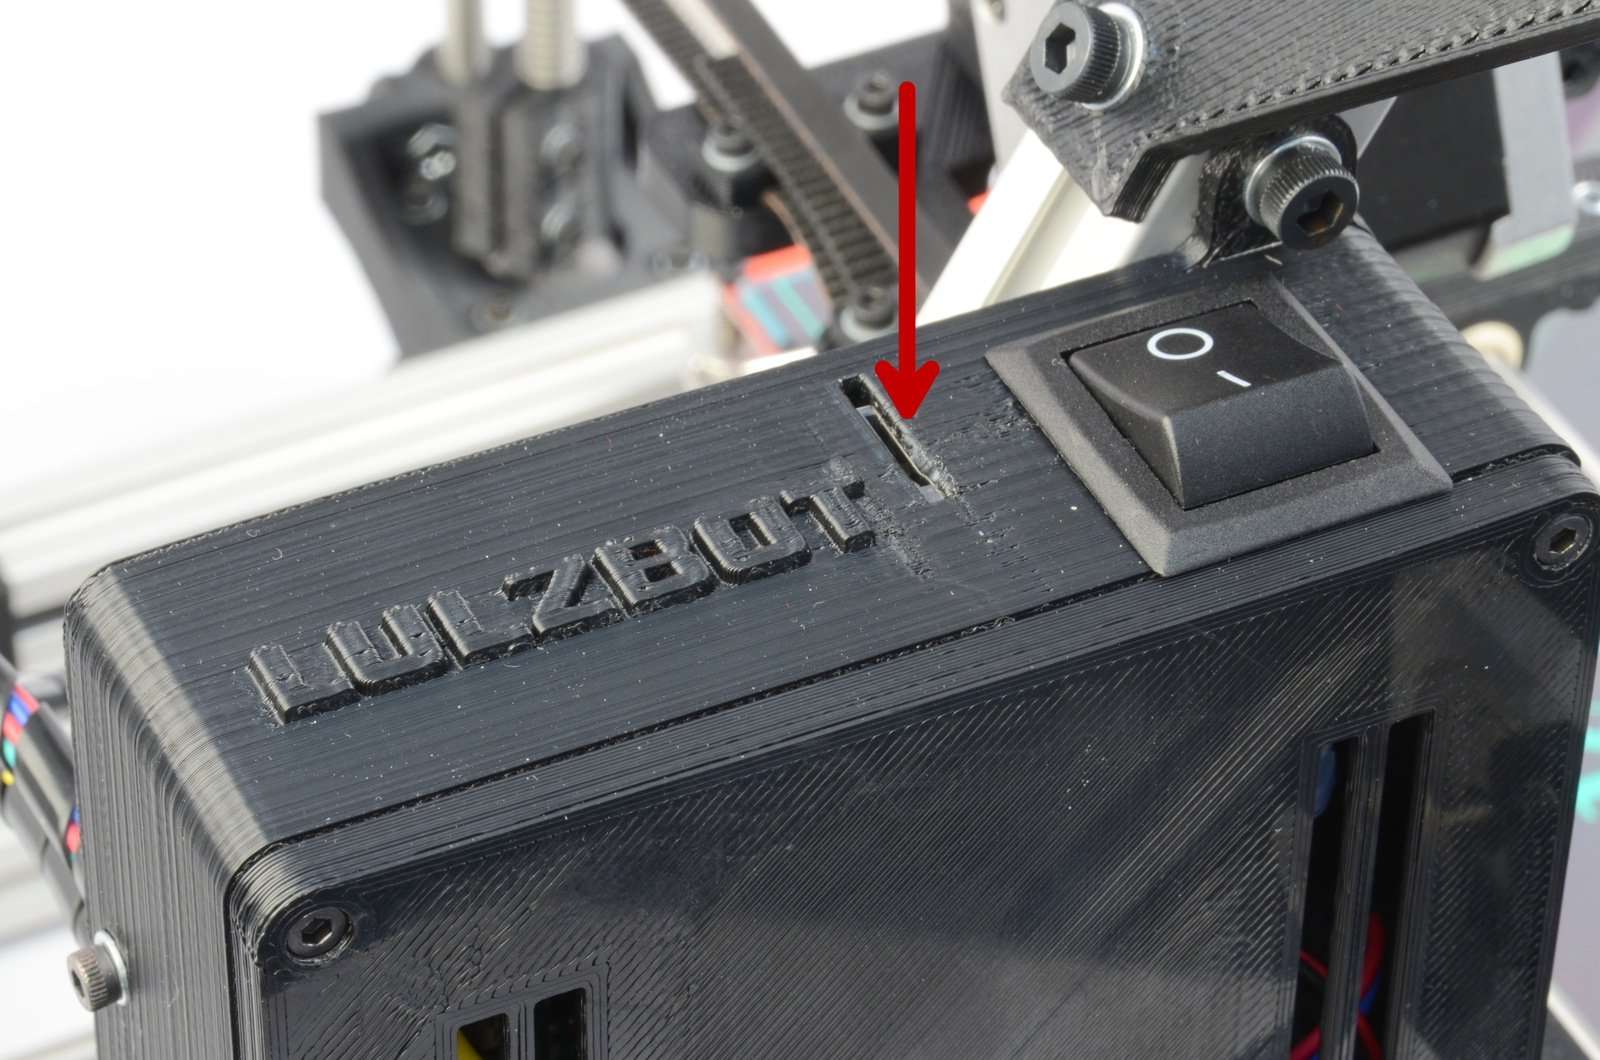
\includegraphics[keepaspectratio=true,angle=0,height=0.4\textheight,width=1.0\textwidth]{sdramps.jpg}
\caption{SDRAMPS}
\label{fig:sdramps}
\end{figure}

\end{enumerate}
